\documentclass[11pt,a4paper]{article}

\PassOptionsToPackage{a4paper,margin=24mm,headheight=14pt}{geometry}
\PassOptionsToPackage{hidelinks}{hyperref}
\usepackage{standards}
\usepackage{lmodern}
\usepackage{array}
\usepackage{tabularx}
\usepackage{longtable}
\usepackage{wrapfig}
\usepackage{multicol}
\usetikzlibrary{arrows.meta,positioning,fit,calc,backgrounds,matrix}
\graphicspath{{images_datasets/}}

\definecolor{ink}{RGB}{32,44,58}
\definecolor{accent}{RGB}{37,96,151}
\definecolor{soft}{RGB}{237,243,248}
\definecolor{warning}{RGB}{139,69,19}
\setlength{\parindent}{0pt}
\setlength{\parskip}{6pt}
\setlist[itemize]{leftmargin=18pt,itemsep=2pt,topsep=3pt}
\renewcommand{\arraystretch}{1.18}
\captionsetup{font=small,labelfont=bf}
\lstset{
  language=Python,
  basicstyle=\ttfamily\footnotesize,
  keywordstyle=\color{accent}\bfseries,
  commentstyle=\color{gray},
  stringstyle=\color{warning},
  backgroundcolor=\color{soft},
  frame=single,
  rulecolor=\color{accent!45},
  breaklines=true,
  showstringspaces=false,
  columns=fullflexible,
  keepspaces=true,
  aboveskip=8pt,
  belowskip=8pt
}

\newcommand{\code}[1]{\texttt{#1}}
\newcommand{\figpath}[1]{../../comparison/output/#1}
\newcommand{\archbox}[2]{\fcolorbox{accent}{soft}{\parbox{#1}{\centering #2}}}
\newcommand{\resultbox}[1]{%
  \vspace{3pt}\noindent
  \fcolorbox{accent}{soft}{\parbox{0.94\textwidth}{#1}}\vspace{4pt}}
\newcommand{\twographs}[6]{%
\begin{figure}[H]
\centering
\begin{minipage}[t]{0.48\textwidth}
\centering
\includegraphics[width=\linewidth]{\figpath{#1}}
\captionof{subfigure}{#2}
\end{minipage}\hfill
\begin{minipage}[t]{0.48\textwidth}
\centering
\includegraphics[width=\linewidth]{\figpath{#3}}
\captionof{subfigure}{#4}
\end{minipage}
\caption{#5}
\label{#6}
\end{figure}}
\newcommand{\maskedscoremat}{%
\begin{array}{c@{\;}c}
& \begin{array}{ccc} \mathbf{k}_1 & \mathbf{k}_2 & \mathbf{k}_3 \end{array}\\[-1mm]
\begin{array}{c} \mathbf{q}_1\\[1.8mm] \mathbf{q}_2\\[1.8mm] \mathbf{q}_3 \end{array}
&
\begin{bmatrix}
s_{11} & s_{12} & s_{13}\\
-\infty & s_{22} & s_{23}\\
-\infty & -\infty & s_{33}
\end{bmatrix}
\end{array}}
\newcommand{\alphamat}{\begin{bmatrix}
 \alpha_{11} & \alpha_{12} & \alpha_{13}\\
 0 & \alpha_{22} & \alpha_{23}\\
 0 & 0 & \alpha_{33}
\end{bmatrix}}

\title{\textbf{Vision-Language Model Comparison}}
\author{Sam}
\date{}

\begin{document}
\maketitle

\begin{abstract}
This project develops a common benchmark harness for comparing
vision-language models across visual question answering, captioning,
detection, classification, preference, rating, and prompt-reconstruction
tasks. The final evaluation focuses on hosted API models using 20 examples
per benchmark and identical execution settings. GPT-4o and Claude Sonnet 4.5
are compared on 36 jointly completed benchmarks; GPT-4o wins 22, Claude wins
10, and 4 are tied. A second comparison covers the 21 benchmarks completed
by GPT-4o, GPT-4.1, GPT-5, Gemini 3.5 Flash, and Claude Sonnet 4.5. GPT-4o
leads overall and in captioning, GPT-4.1 leads visual question answering,
and Claude leads detection. The results show that model rankings depend on
task family and that matched benchmark coverage is necessary for fair
aggregation. Because each benchmark uses a small sample and hosted models
may change, the conclusions should be interpreted as a reproducible
experimental snapshot rather than a permanent leaderboard.
\end{abstract}

\tableofcontents
\clearpage

\section{Introduction and Motivation}

\section{Objectives}

\section{Transformer Background}

A Transformer is a neural-network architecture designed to process a sequence
of tokens while allowing every token to gather information from other relevant
tokens. It was introduced for machine translation by
Vaswani et al.~\cite{vaswani2017attention}, but the same basic design now
underpins most large language and vision-language models. In a text model, the
tokens are usually pieces of words. In a vision-language model, image patches
or features are also converted into vectors that can be processed alongside
text. The important point is that, after this conversion, both modalities can
be handled as sequences of numerical representations.

The first step is an embedding. Each token is mapped to a vector, and
positional information is added so that the model can distinguish, for
example, the first word from the tenth word or one image patch from another.
The vectors then pass through a stack of Transformer blocks. Each block
contains an attention operation, a small feed-forward network applied to each
position, residual connections that preserve earlier information, and layer
normalisation that stabilises training. Repeating this process gradually turns
simple token vectors into context-aware representations.

\begin{figure}[H]
\centering

\includegraphics[width=\textwidth,height=0.76\textheight,keepaspectratio]
  {../gpt3_attention_block_input_outside_dashed.pdf}
\caption{A complete masked self-attention block. The input vectors are
projected into queries, keys, and values before attention scores are computed.}
\label{fig:attention-overview}
\end{figure}

Self-attention is the central mechanism. From each input vector
\(\mathbf{z}_i\), the model learns three projections: a query
\(\mathbf{q}_i\), a key \(\mathbf{k}_i\), and a value \(\mathbf{v}_i\).
Queries describe what a position is looking for, keys describe what each
position offers, and values contain the information that may be passed
onward. Compatibility is measured with a scaled dot product:
\[
  s_{ij} = \frac{\mathbf{q}_i\mathbf{k}_j^\top}{\sqrt{d_k}},
  \qquad
  \alpha_{ij} = \operatorname{softmax}_j(s_{ij}).
\]
The division by \(\sqrt{d_k}\) prevents large vector dimensions from producing
extreme softmax values. The attention weights \(\alpha_{ij}\) are then used
to form a weighted sum of the value vectors. Put simply, the model decides
which earlier pieces of the input matter and how much of each one to carry
forward.

The diagrams show \emph{masked} attention, as used by autoregressive language
models. The causal mask prevents a token from reading tokens that have not yet
been generated. Thus, when predicting the next token, the model may use the
prompt and its earlier output but cannot look into the future. Several
attention heads perform this operation in parallel. Different heads can focus
on different relationships, such as nearby syntax, a distant name, an object
in an image, or the connection between a question and a visual region. Their
outputs are concatenated and projected before entering the rest of the block.

During training, model parameters are adjusted to reduce prediction error over
large collections of examples. During inference, the trained Transformer
receives the image and prompt, processes them through its blocks, and predicts
output tokens one at a time. The models evaluated in this project differ
substantially in scale, training data, visual encoders, alignment methods, and
serving infrastructure, but this attention-based processing is the common
architectural idea behind them.

\section{Planning}

The project was carried out between February and June 2026. The initial
plan divided the work sequentially into background study, implementation,
experimentation, and writing. In practice, benchmark implementation and
dataset validation required more time than expected. The experimental and
writing phases therefore overlapped, and the final API evaluations were run
in parallel during the preparation of this report.

\begin{table}[H]
\centering
\small
\caption{Original and final project planning. The effort values are a
retrospective estimate of effective working time.}
\label{tab:project-planning}
\begin{tabularx}{\textwidth}{@{}p{3.2cm}p{2.4cm}p{2.7cm}rX@{}}
\toprule
\textbf{Task} & \textbf{Original plan} & \textbf{Final execution} &
\textbf{Hours} & \textbf{Main outputs} \\
\midrule
Requirements and literature review
& February
& 24 February--15 March
& 35
& Scope, model taxonomy, task types, and initial dataset selection. \\

Architecture and prototype
& February--March
& 1--31 March
& 45
& Common model interface, first benchmark runners, and an initial user
interface. \\

Dataset and benchmark implementation
& March--April
& 16 March--19 May
& 110
& Dataset adapters, eight benchmark families, result serialization, and
dataset-specific corrections. \\

Model integration and API orchestration
& April
& 7 May--10 June
& 55
& Local-model wrappers, hosted-model wrappers, resumable notebooks, and
parallel isolated API runs. \\

Evaluation, debugging, and reruns
& April--May
& 8 May--10 June
& 65
& Smoke tests, full benchmark runs, telemetry, error diagnosis, and
re-execution of accessible datasets. \\

Exploratory fine-tuning
& May
& 20 May--10 June
& 30
& Fashion-MNIST experiments and an eight-task LLaVA-OneVision LoRA
pipeline, retained as exploratory work rather than part of the final
comparison. \\

Analysis and report preparation
& May
& 27 May--10 June
& 40
& Matched API-model comparisons, plots, uncertainty analysis, discussion,
and final report. \\
\midrule
\textbf{Total}
& \textbf{February--May}
& \textbf{24 February--10 June}
& \textbf{380}
& \textbf{Approximately 9.5 full-time working weeks.} \\
\bottomrule
\end{tabularx}
\end{table}

The principal deviation from the original plan was the extension of
benchmark engineering into May and June. Differences between dataset
schemas, unavailable samples, provider rate limits, and long-running API
requests made a strictly sequential execution impractical. The revised plan
reduced schedule risk by running one isolated process per API model, saving
each completed benchmark immediately, and performing analysis on partial
results while the remaining evaluations continued. The final report was
narrowed to the API models with sufficient matched coverage; the local
fine-tuning pipeline remains documented as exploratory implementation work
and is not included in the reported model rankings.

\section{Costs}

This cost estimate is intentionally limited to the compute services required
to reproduce the API benchmarks currently being executed and the
LLaVA-OneVision fine-tuning experiment. It excludes development labour,
the existing workstation, Internet access, and free/open-source software
licences. Prices are stated in US dollars before tax and were checked on
10 June 2026.

\subsection{Estimation assumptions}

Each API model is evaluated on 44 benchmarks. The notebook uses 20 examples
per benchmark, except UCF101, which uses 9, giving 869 requests per model.
The benchmark result files record latency but not provider token usage.
Consequently, the budget assumes 1.50 million billed input tokens and
0.15 million billed output tokens per complete model run. This deliberately
allows for image tokens, prompts, labels, and short reasoning traces. The
estimated charge is
\[
 C_{\mathrm{API}} =
 1.50P_{\mathrm{input}} + 0.15P_{\mathrm{output}},
\]
where both prices are expressed in dollars per million tokens. Free quotas,
cached-input discounts, batch discounts, and promotional credits are not
deducted, so the figures represent a comparable commercial reproduction
cost rather than the exact account invoice.

\begin{table}[H]
\centering
\small
\caption{Estimated cost of one complete run of the active API benchmark
matrix.}
\label{tab:api-model-costs}
\begin{tabularx}{\textwidth}{@{}Xlrrr@{}}
\toprule
\textbf{Model} & \textbf{Provider} &
\textbf{Input / 1M} & \textbf{Output / 1M} &
\textbf{Estimated run} \\
\midrule
\texttt{gpt-4o} & OpenAI & \$2.50 & \$10.00 & \$5.25 \\
\texttt{gpt-4.1} & OpenAI & \$2.00 & \$8.00 & \$4.20 \\
\texttt{gpt-5} & OpenAI & \$1.25 & \$10.00 & \$3.38 \\
\texttt{claude-sonnet-4-5} & Anthropic & \$3.00 & \$15.00 & \$6.75 \\
\texttt{gemini-3.5-flash} & Google & \$2.70 & \$16.20 & \$6.48 \\
\texttt{qwen3.5-plus} & Alibaba Cloud, Singapore & \$0.40 & \$2.40 & \$0.96 \\
\midrule
\multicolumn{4}{r}{\textbf{API subtotal}} & \textbf{\$27.02} \\
\bottomrule
\end{tabularx}
\end{table}

The rates come from the providers' published pricing pages:
OpenAI\footnote{\url{https://openai.com/api/pricing/}},
Anthropic\footnote{\url{https://platform.claude.com/docs/en/about-claude/pricing}},
Google\footnote{\url{https://ai.google.dev/gemini-api/docs/pricing}}, and
Alibaba Cloud Model Studio\footnote{\url{https://www.alibabacloud.com/help/en/model-studio/model-pricing}}.
Alibaba's one-million-token introductory quota could reduce the first Qwen
run, but it is omitted because it is temporary and account-dependent.



\section{Experimental Methodology}

Benchmarking is more than collecting a single accuracy number. Broad suites
such as MMLU and BIG-bench demonstrate why many tasks are needed to expose
uneven capabilities~\cite{hendrycks2020mmlu,srivastava2022bigbench}, while
HELM argues for standardised scenarios, multiple metrics, and transparent
prompts and outputs~\cite{liang2022helm}. Dynabench further shows that static
test sets can become less informative as models adapt to them and motivates
evaluation that evolves with model failures~\cite{kiela2021dynabench}.

For multimodal systems, benchmark breadth must include both perception and
reasoning. MMMU illustrates this with questions spanning many disciplines and
visual formats~\cite{yue2023mmmu}. System quality is also not only predictive
quality: MLPerf formalises reproducible latency and throughput measurement
under controlled run rules~\cite{reddi2019mlperf}. Finally, public benchmark
examples may appear in model training data, so apparently strong results can
partly reflect memorisation rather than generalisation
~\cite{li2023contamination}. These principles motivate the matched benchmark
intersection, task-family reporting, runtime telemetry, saved raw outputs,
and cautious interpretation used in this project.

\subsection{Datasets}
\subsubsection{Dataset selection procedure}

For each period $\{$pre-2015, 2015, 2016, \dots, 2024, 2025$\}$, I selected the three multimodal datasets with the highest number of citations on \texttt{Semantic Scholar} (\texttt{semanticscholar.org/}) as Google scholar does not allow me to order items by number of citations. Concretely, for each year bin I queried \texttt{Semantic Scholar} with the keywords \texttt{``dataset''}, \texttt{``image''}, and \texttt{``objects''} and then ranked results by the number of citations reported by the Semantic Scholar platform~\cite{kinney2023semanticscholar}. A dataset was included only if it satisfied all of the following:

\begin{enumerate}
  \item \textbf{Search visibility.} The dataset must appear in \texttt{Semantic Scholar} search results for at least one of the keywords \emph{dataset}, \emph{image}, or \emph{objects}.
  \item \textbf{Multimodality with vision.} The dataset must be multimodal and include \textbf{images or videos}. Purely non-visual multimodal datasets are excluded (e.g., ESC (2015) is excluded because it focuses on audio). Datasets with 3D/geometry are acceptable \textbf{if} they also include 2D images or videos (e.g., FlyingThings3D (2015) qualifies); datasets lacking a 2D visual modality are excluded (e.g., Google Scanned Objects (2022) excluded).
  \item \textbf{Scope exclusions.} The dataset must \textbf{not} be:
    \begin{itemize}
      \item fully medical (e.g., CheXpert (2019) excluded),
      \item exclusively aerial/remote-sensing imagery (e.g., EuroSAT (2017) excluded),
      \item images or videos taken from vehicles' cameras (e.g., nuScenes (2019) excluded;\, HDR cameras on top of vehicles such as the ones used for the street view on Google Maps are OK, hence Cityscapes (2016) is included).
    \end{itemize}
\end{enumerate}

Applying these rules, I retained, for each period, the top three qualifying datasets by publication count.

Every selected source is wrapped by a dataset adapter that converts its native
schema into the common fields expected by the benchmarks. This is necessary
because even apparently simple concepts such as ``image'' and ``caption'' are
stored under different keys, formats, and access mechanisms. For example,
Conceptual Captions often supplies an image URL rather than an already decoded
image. Listing~\ref{lst:dataset-adapter} shows how the real adapter skips
unavailable URLs and returns a uniform RGB image and caption record.

\begin{lstlisting}[caption={Dataset standardisation from
\texttt{dataset/conceptual\_captions.py}.},label={lst:dataset-adapter}]
def get_available_samples(self, n):
    samples = []
    for raw_row in self.ds:
        row = self._standardize_row(raw_row)
        try:
            row["image"] = self.get_image_from_row(row)
        except Exception:
            continue
        samples.append(row)
        if len(samples) >= n:
            break
    return samples

def get_image_from_row(self, row):
    image_url = str(row.get("image_url", "")).strip()
    request = Request(
        image_url, headers={"User-Agent": "Mozilla/5.0"}
    )
    with urlopen(request, timeout=10) as response:
        return Image.open(BytesIO(response.read())).convert("RGB")
\end{lstlisting}




































































\subsubsection{Summary of the Datasets as a Whole}

\noindent\textbf{Abbreviations.}
Licenses: \textbf{FNCR} = free for non-commercial research; \textbf{FAP} = free for any purpose; \textbf{MRL} = Meta Research License; \textbf{OC} = original copyright; \textbf{Unk.} = unknown. Standard license identifiers such as CC BY, CC0, MIT, Apache-2.0, and GPL-3.0 are retained.
Elements: \textbf{Img} = images; \textbf{Vid} = videos; \textbf{Lbl} = labels; \textbf{Act} = action labels; \textbf{Seg} = segmentation; \textbf{Cap} = captions; \textbf{BB} = bounding boxes; \textbf{Rel} = relationships; \textbf{QA} = question--answer pairs; \textbf{Aud} = audio; \textbf{Txt} = text; \textbf{Pr} = prompts; \textbf{Sc} = scores; \textbf{Pref} = preference.
Evaluation types: \textbf{A} = answering questions; \textbf{B} = bounding box object detection; \textbf{C} = captioning; \textbf{E} = editing prompt reconstruction; \textbf{G} = generating prompt reconstruction; \textbf{L} = labeling; \textbf{P} = preference; \textbf{R} = rating.


\begin{table}[H]
\centering
\caption{Pre-2015 publications.}
\label{tab:datasets}
\begin{tabular}{p{2.5cm}p{1.65cm}p{3.05cm}p{3.2cm}p{2.15cm}}
\hline
\textbf{Name} & \textbf{Citations} & \textbf{License} & \textbf{Elements} & \textbf{Eval.}\\
\hline
ImageNet~\cite{deng2009imagenet} & 66,633 & FNCR & Img + Lbl & L\\
\hline
UCF101~\cite{soomro2012ucf101} & 6,460 & CC0-1.0 & Vid + Act & L\\
\hline
MS COCO~\cite{lin2014coco} & 46,361 & CC BY 4.0 & Img + Seg + Cap & B + C\\
\hline

\end{tabular}
\end{table}

\begin{table}[H]
\centering
\caption{2015 publications.}
\begin{tabular}{p{2.5cm}p{1.65cm}p{3.05cm}p{3.2cm}p{2.15cm}}
\hline
\textbf{Name} & \textbf{Citations} & \textbf{License} & \textbf{Elements} & \textbf{Eval.}\\
\hline
Flickr30k Entities~\cite{plummer2015flickr30k} & 2,226 & FNCR & Img + Cap + BB + Rel & B + C\\
\hline
FlyingThings3D~\cite{mayer2016large} & 2,758 & FNCR & Img pairs + 3D & A\\
\hline
LSUN~\cite{yu2015lsun} & 2,436 & FNCR + conditions & Img + Lbl & L\\
\hline

\end{tabular}
\end{table}

\begin{table}[H]
\centering
\caption{2016 publications.}
\begin{tabular}{p{2.5cm}p{1.65cm}p{3.05cm}p{3.2cm}p{2.15cm}}
\hline
\textbf{Name} & \textbf{Citations} & \textbf{License} & \textbf{Elements} & \textbf{Eval.}\\
\hline
Cityscapes~\cite{cordts2016cityscapes} & 12,189 & FNCR & Img + Seg + Lbl & L\\
\hline
Visual Genome~\cite{krishna2017visualgenome} & 6,018 & CC BY 4.0* & Img + BB + Rel + QA & A\\
\hline
VQA v2.0~\cite{goyal2017vqa} & 3,558 & CC BY 4.0 & Img pairs + QA & A\\
\hline

\end{tabular}
\end{table}

\begin{table}[H]
\centering
\caption{2017 publications.}
\begin{tabular}{p{2.5cm}p{1.65cm}p{3.05cm}p{3.2cm}p{2.15cm}}
\hline
\textbf{Name} & \textbf{Citations} & \textbf{License} & \textbf{Elements} & \textbf{Eval.}\\
\hline
Fashion-MNIST~\cite{xiao2017fashionmnist} & 9,435 & MIT & Img + Lbl & L\\
\hline
Kinetics Human Action Video Dataset~\cite{kay2017kinetics} & 3,981 & CC BY 4.0* & Vid + Lbl & L\\
\hline
iNaturalist~\cite{vanhorn2018inaturalist} & 1,763 & CC BY-NC & Img + BB + Lbl & L + B\\
\hline

\end{tabular}
\end{table}

\begin{table}[H]
\centering
\caption{2018 publications.}
\begin{tabular}{p{2.5cm}p{1.65cm}p{3.05cm}p{3.2cm}p{2.15cm}}
\hline
\textbf{Name} & \textbf{Citations} & \textbf{License} & \textbf{Elements} & \textbf{Eval.}\\
\hline
Places~\cite{zhou2017places} & 4,319 & FNCR & Img + Lbl & L\\
\hline
Conceptual Captions~\cite{sharma2018conceptual} & 2,643 & FAP & Img + Cap & C\\
\hline
Open Images V4~\cite{kuznetsova2020openimages} & 1,441 & CC BY 2.0 (Img) / 4.0 (ann.) & Img + BB + Lbl + Rel & L + B\\
\hline

\end{tabular}
\end{table}

\begin{table}[H]
\centering
\caption{2019 publications.}
\begin{tabular}{p{2.5cm}p{1.65cm}p{3.05cm}p{3.2cm}p{2.15cm}}
\hline
\textbf{Name} & \textbf{Citations} & \textbf{License} & \textbf{Elements} & \textbf{Eval.}\\
\hline
GQA~\cite{hudson2019gqa} & 2,402 & CC BY 4.0 & Img + QA & A\\
\hline
MVTec AD~\cite{bergmann2019mvtec} & 1,549 & CC BY-NC-SA 4.0 & Img + Seg & L\\
\hline
LVIS~\cite{gupta2019lvis} & 1,492 & CC BY 4.0 & Img + Seg + Lbl & B\\
\hline

\end{tabular}
\end{table}

\begin{table}[H]
\centering
\caption{2020 publications.}
\begin{tabular}{p{2.5cm}p{1.65cm}p{3.05cm}p{3.2cm}p{2.15cm}}
\hline
\textbf{Name} & \textbf{Citations} & \textbf{License} & \textbf{Elements} & \textbf{Eval.}\\
\hline
DocVQA~\cite{mathew2020docvqa} & 930 & Unk. & Img + QA & A\\
\hline
DFDC~\cite{dolhansky2020dfdc} & 597 & MRL? & Vid + Lbl & L\\
\hline
TextCaps~\cite{sidorov2020textcaps} & 469 & CC BY 4.0 & Img + Cap & C\\
\hline

\end{tabular}
\end{table}

\begin{table}[H]
\centering
\caption{2021 publications.}
\begin{tabular}{p{2.5cm}p{1.65cm}p{3.05cm}p{3.2cm}p{2.15cm}}
\hline
\textbf{Name} & \textbf{Citations} & \textbf{License} & \textbf{Elements} & \textbf{Eval.}\\
\hline
LAION-400M~\cite{schuhmann2021laion400m} & 1,486 & CC BY 4.0 (meta.); Img: OC & Img + Lbl + Sc & C\\
\hline
FairFace~\cite{karkkainen2021fairface} & 616 & CC BY 4.0 & Img + Lbl & L\\
\hline
HDTF~\cite{zhang2021hdtf} & 413 & GPL-3.0 & Vid + Aud + Txt & C\\
\hline

\end{tabular}
\end{table}

\begin{table}[H]
\centering
\caption{2022 publications.}
\begin{tabular}{p{2.5cm}p{1.65cm}p{3.05cm}p{3.2cm}p{2.15cm}}
\hline
\textbf{Name} & \textbf{Citations} & \textbf{License} & \textbf{Elements} & \textbf{Eval.}\\
\hline
LAION-5B~\cite{schuhmann2022laion5b} & 4,059 & CC BY 4.0 (meta.); Img: OC & Img + Cap + Sc & C\\
\hline
DiffusionDB~\cite{wang2022diffusiondb} & 349 & CC0-1.0 (data) / MIT (code) & Img + Pr + Sc & G\\
\hline
TAD66K~\cite{he2022tad66k} & 111 & Apache-2.0 & Img + Sc & R\\
\hline

\end{tabular}
\end{table}

\begin{table}[H]
\centering
\caption{2023 publications.}
\begin{tabular}{p{2.5cm}p{1.65cm}p{3.05cm}p{3.2cm}p{2.15cm}}
\hline
\textbf{Name} & \textbf{Citations} & \textbf{License} & \textbf{Elements} & \textbf{Eval.}\\
\hline
MagicBrush~\cite{zhang2023magicbrush} & 391 & CC BY-SA 4.0 & Img pairs + edit Pr & E\\
\hline
Pick-a-Pic~\cite{kirstain2023pickapic} & 559 & Unk. & Img + Pr + Pref & P\\
\hline
InternVid~\cite{wang2023internvid} & 411 & CC BY-NC-SA 4.0 & Vid + Cap & C\\
\hline

\end{tabular}
\end{table}

\begin{table}[H]
\centering
\caption{2024 publications.}
\begin{tabular}{p{2.5cm}p{1.65cm}p{3.05cm}p{3.2cm}p{2.15cm}}
\hline
\textbf{Name} & \textbf{Citations} & \textbf{License} & \textbf{Elements} & \textbf{Eval.}\\
\hline
OpenVid-1M~\cite{nan2024openvid} & 149 & Unk. & Vid + Pr + Cap & C + G\\
\hline
Visual CoT~\cite{shao2024visualcot} & 148 & CC BY-SA 4.0 & Img + BB + QA & A + B\\
\hline
HQ-Edit~\cite{hui2024hqedit} & 104 & CC BY-NC-4.0 & Img pairs + edit Pr & E\\
\hline

\end{tabular}
\end{table}

\begin{table}[H]
\centering
\caption{2025 publications.}
\begin{tabular}{p{2.5cm}p{1.65cm}p{3.05cm}p{3.2cm}p{2.15cm}}
\hline
\textbf{Name} & \textbf{Citations} & \textbf{License} & \textbf{Elements} & \textbf{Eval.}\\
\hline
BLIP3o-60k~\cite{chen2025blip3o} & 91 & Apache-2.0 & Img + Pr & G\\
\hline
ImgEdit~\cite{ye2025imgedit} & 38 & Apache-2.0 & Img pairs + edit Pr & E\\
\hline
ShareGPT-4o-Image~\cite{chen2025sharegpt} & 27 & Apache-2.0 & Img + Pr & G + E\\
\hline
\end{tabular}
\end{table}


In the dataset summary tables, when images are grouped or classified into categories, we count this as having \bfit{labels}. Labels are category tags that describe what the image or video shows. For example, a picture of a dog in \textbf{ImageNet} has labels such as \texttt{dog}, \texttt{mammal}, \texttt{animal}, while a picture of a woman laughing in \textbf{UCF101} is labeled as \texttt{smiling}.  \bfit{Captions} go a step further by describing what is happening or what can be seen in the image or video, as seen in Figure~\ref{fig:conceptual-captions} for an image captioned "\texttt{pop artist performs at the festival in a city}" in the \textbf{Conceptual Captions} dataset.\bfit{Prompts} are pieces of text used to generate or edit images in datasets built around generative models. Examples can be seen in Figures~\ref{fig:diffusiondb} or \ref{fig:magicbrush} for the \textbf{DiffusionDB} or \textbf{MagicBrush} datasets respectively.\\

\bfit{Bounding boxes} pinpoint specific object instances within an image by drawing rectangles around them (using coordinates such as $(x_{\min},y_{\min},x_{\max},y_{\max})$). See Figures \ref{fig:flickr30k} or \ref{fig:visual-genome} from \textbf{Flickr30K} or \textbf{Visual Genome} respectively as examples. \bfit{Segmentation} goes a step further by outlining the exact shape of each object, assigning every pixel to a class or instance. Semantic segmentation labels each pixel by class, while instance segmentation gives each object its own mask. See Figures \ref{fig:mscoco} or \ref{fig:cityscapes} from \textbf{MS COCO} or \textbf{Cityscapes} respectively for examples.\\

Finally, \textbf{Pick-a-Pic} captures human \bfit{preferences} for images generated by text-to-image diffusion models. Images in the dataset come in pairs, with one of the two image being preferred. Figure~\ref{fig:pickapic2} shows examples where the chosen image is highlighted and the rejected one is darkened. The term \bfit{scores} refers to any numerical metadata. For example, an aesthetic score as in \textbf{TAD66K} or an NSFW score as in \textbf{LAION-5B}. \bfit{QA-pairs} (question–answer pairs) are exactly what they sound like: a question about the image and its corresponding answer, such as “\texttt{What type of fruit in the image is round?}” and “\texttt{apple}”, as shown in Figure \ref{fig:gqa} for the \textbf{GQA} dataset.\\


 \bfit{Relationships} refer to datasets that explicitly describe how objects interact or relate to one another, rather than just listing them. Only two datasets meet this criterion: \textbf{Flickr30K Entities} and \textbf{Visual Genome}. The former connects phrases in captions that refer to the same entity (like “\texttt{a boy}” and “\texttt{the child}”) and links them to specific bounding boxes in the image, as shown in Figure~\ref{fig:flickr30k}. The latter represents scenes as graphs of objects and their relationships e.g., “\texttt{man \textit{riding} horse}”, as shown in Figure~\ref{fig:visual-genome}. Finally, when a dataset contains \bfit{3D data}, it includes information about the geometry of the scene beyond standard RGB images. This only applies to \textbf{FlyingThings3D}, which contains stereo image pairs (left and right views rendered from two virtual cameras) along with detailed geometric information such as depth (disparity) maps, optical flow, segmentation masks, material indices, motion boundaries, and camera calibration data. Together, these describe the full 3D structure and motion of the scene, as shown in Figure~\ref{fig:flyingthings3d}.\\

Regarding the licenses,

\clearpage
\subsubsection{Detailed Dataset Catalogue}
\begin{multicols}{2}

\begin{figure*}[t]
    \centering
    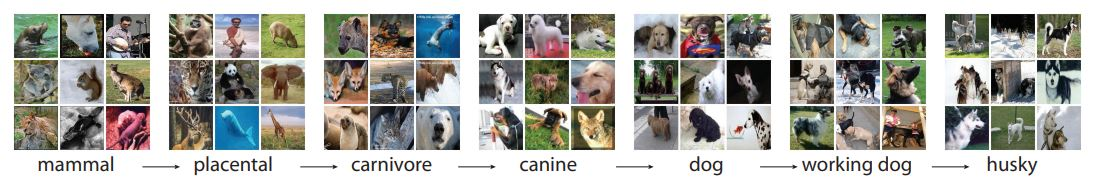
\includegraphics[width=\textwidth]{ImageNet.JPG}
    \caption{Example of ImageNet hierarchical organization, showing a path from \textit{mammal} to \textit{husky}.}
\end{figure*}

\textbf{ImageNet}~\cite{deng2009imagenet} is a large-scale database of human-annotated photographs organized into a hierarchy of visual concepts. Each category, or “synset,” groups together images of the same concept, such as "husky", and is linked to related categories within a larger hierarchy, such as "animal".  
At the time of publication, ImageNet contained 12 major groups, covering 5,247 categories and about 3.2 million images.\\

















\begin{figure}[H]
    \centering
    \vspace{-10pt}
    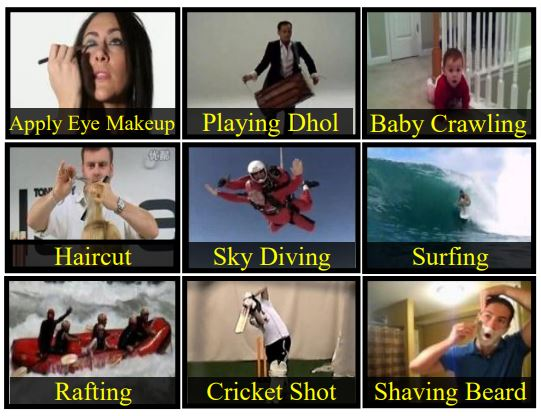
\includegraphics[width=0.5\textwidth]{UCF101.JPG}
    \caption{Sample frames from UCF101 showing diverse action classes such as \textit{Apply Eye Makeup}, \textit{Playing Dhol}, and \textit{Baby Crawling}.}
    \vspace{-10pt}
    \label{fig:ucf101}
\end{figure}

\textbf{UCF101 (2012)}~\cite{soomro2012ucf101}. The University of Central Florida (UCF) compiled a total of 13,320 video clips amounting to about 27 hours of footage. Each clip was then labeled as one of 101 action classes, 51 of which preserved audio. The videos are stored at a resolution of 320×240 pixels and 25 frames per second. On average, clips are about 7 seconds long.\\ 



















\begin{figure}[H]
    \centering
    \vspace{-10pt}
    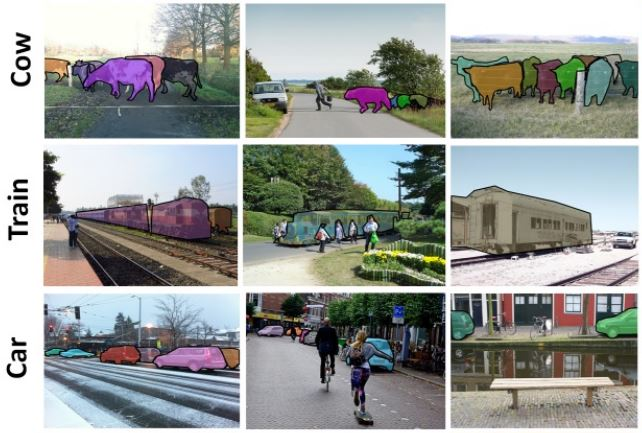
\includegraphics[width=0.5\textwidth]{MSCOCO.JPG}
    \caption{Examples from the MS COCO dataset showing object segmentations for categories such as \textit{cow}, \textit{train}, and \textit{car}}
    \vspace{-10pt}
    \label{fig:mscoco}
\end{figure}


\textbf{Microsoft COCO (2014)}~\cite{lin2014coco}. The Microsoft COCO, abbreviated MS COCO, dataset contains photographs of everyday environments filled with multiple objects in their natural context. Each object instance is carefully annotated with detailed segmentations, allowing precise localization within the image as shown in Figure~\ref{fig:mscoco}.

MS COCO includes 91 common object categories that are easily recognizable, with over 2.5 million labeled instances across 328,000 images.\\











































\begin{figure}[H]
    \centering
    \vspace{-10pt}
    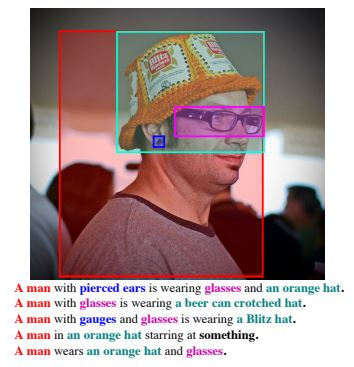
\includegraphics[width=0.35\textwidth]{Flickr30k1.JPG}
    \caption{Example image with captions; phrases in the same color are coreferent and linked to their corresponding bounding boxes.}
    \label{fig:flickr30k}
    \vspace{-10pt}
\end{figure}

\textbf{Flickr30k Entities}~\cite{plummer2015flickr30k} extends the Flickr30k dataset by providing detailed links between image regions and textual phrases. With 31{,}783 images and 158{,}915 captions, the dataset connects mentions that refer to the same entity across captions describing the same image, forming about 244{,}000 coreference chains, and associates these with roughly 276{,}000 manually drawn bounding boxes. An example of the final annotated data is shown in Figure~\ref{fig:flickr30k}, where color-coded phrases correspond to specific image regions.  These annotations enable the new task of \emph{phrase localization}: given an image and a caption, predict the region that corresponds to a particular entity mention.  
























\begin{figure}[H]
    \centering
    \vspace{-10pt}
    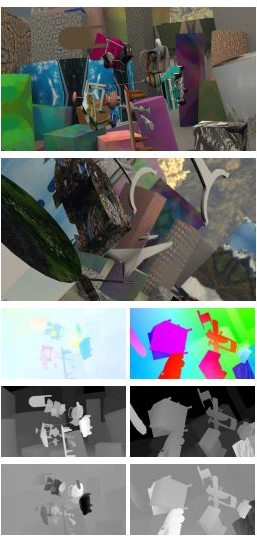
\includegraphics[width=0.5\textwidth]{FlyingThings3D2.jpg}
    \caption{Example scenes from the \textit{FlyingThings3D} dataset. The third row shows optical flow images, the fourth row shows disparity images, and the fifth row shows disparity change images (normalized for display).}
    \label{fig:flyingthings3d}
    \vspace{-10pt}
\end{figure}


\textbf{FlyingThings3D}~\cite{mayer2016large} consists of roughly 25,000 stereo frames rendered using \textit{Blender}, each displaying a  random arrangement of textured 3D objects. Each frame provides left and right RGB images, together with corresponding maps for optical flow, disparity, and disparity change, as well as object segmentation masks, material indices, and motion boundaries as shown in Figure~\ref{fig:flyingthings3d}. Complete camera calibration data and 3D geometry information are also provided.  \\














\begin{figure*}[t]
    \centering
    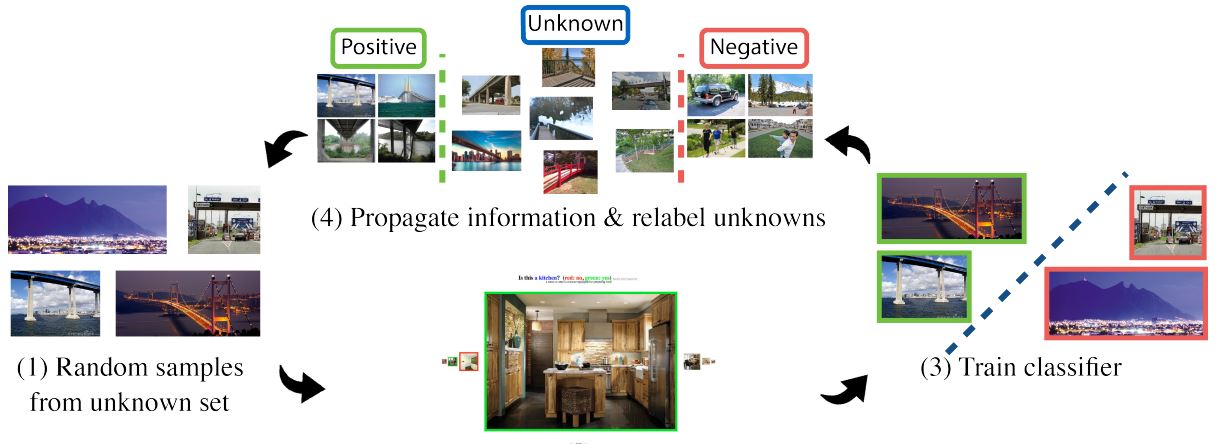
\includegraphics[width=\textwidth]{LSUN.JPG}
    \caption{Example images and scene categories from the \textit{LSUN} dataset.}
    \label{fig:lsun}
\end{figure*}

\textbf{LSUN}~\cite{yu2015lsun} is a very large dataset consisting of about 69 million images belonging to 30 categories. Only a small portion of the images were labeled by humans, the rest being labeled by a trained classifier (e.g., for the \emph{train} category, less than $1/60$ of images were labeled by people), achieving ~90\% precision. Training popular convolutional networks on this larger, if noisier, data leads to noticeable gains; for example, fine-tuning with LSUN reduced a reported classification error from 28.6\% to 22.2\% on a related evaluation.\\





























\begin{figure*}[t]
    \centering
    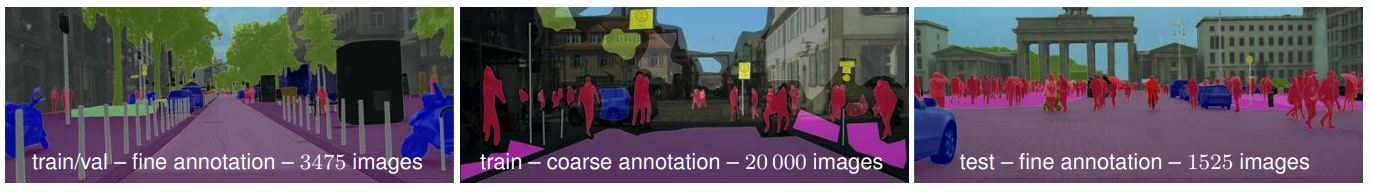
\includegraphics[width=\textwidth]{Cityscapes.JPG}
    \caption{Example scenes from the \textit{Cityscapes} dataset. From left to right: fine annotations for training/validation (3,475 images), coarse annotations for training (20,000 images), and fine annotations for testing (1,525 images). Each image shows dense semantic and instance-level labeling of complex urban street scenes.}
    \label{fig:cityscapes}
\end{figure*}

\textbf{Cityscapes}~\cite{cordts2016cityscapes} contains stereo video sequences recorded across 50 different cities, primarily in Germany. From these recordings, 5,000 images received high-quality fine annotations, while an additional 20,000 were annotated coarsely (less boundary precision) with a ~98\% accuracy after excluding ambiguous (void) regions. Figure~\ref{fig:cityscapes} illustrates examples of both fine and coarse annotations used for training, validation, and testing. The dataset is split into 2,975 training, 500 validation, and 1,525 test images, ensuring balance across geography, population size, and season. In total, 30 semantic classes (19 for evaluation) are grouped into eight high-level categories: flat, construction, nature, vehicle, sky, object, human, and void.  
































\begin{figure*}[t]
    \centering
    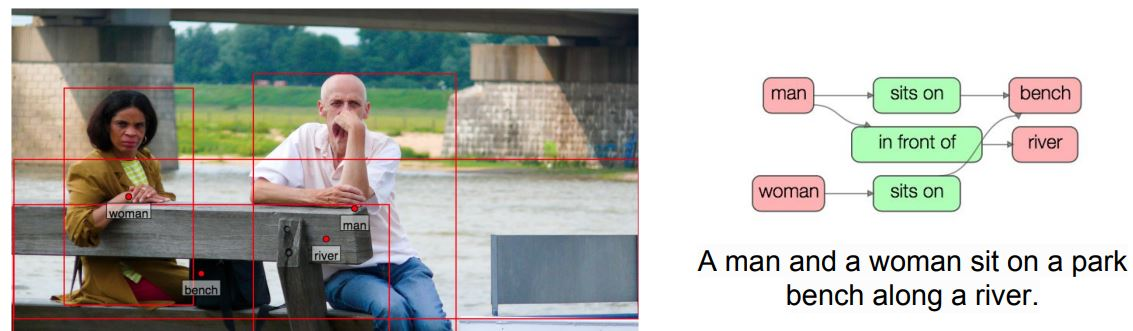
\includegraphics[width=\textwidth]{VisualGenome1.JPG}
    \caption{Example image and scene graph from the \textbf{Visual Genome} dataset. The left side shows labeled objects with bounding boxes, while the right side illustrates the relationships between these objects in a graph.}
    \label{fig:visual-genome}
\end{figure*}

\textbf{Visual Genome}~\cite{krishna2017visualgenome} human-annotated imagea describe not only \emph{what} objects are present, but also \emph{how} they interact. The dataset contains over 100,000 real-world images, each annotated with an average of 21 objects, 18 attributes, and 18 pairwise relationships, as exemplified in Figure ~\ref{fig:visual-genome}. Beyond scene graphs, Visual Genome includes over 1.7 million question–answer pairs designed to test visual reasoning and comprehension. 






























\begin{figure}[H]
    \centering
    \vspace{-10pt}
    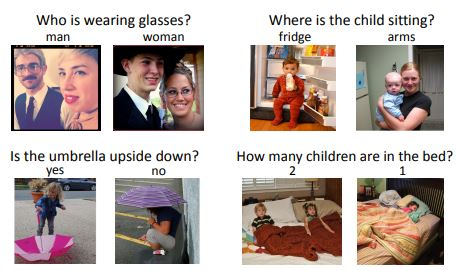
\includegraphics[width=0.5\textwidth]{VQAV2.JPG}
    \caption{Examples from the balanced \textbf{VQA v2.0} dataset. Each question is paired with images that are visually similar yet lead to different answers, encouraging models to use visual evidence rather than language priors.}
    \label{fig:vqa-v2}
    \vspace{-10pt}
\end{figure}


\noindent
\textbf{VQA v2.0}~\cite{goyal2017vqa}. For each image in the Visual Question Answering (VQA) dataset, annotators tried to find a complementary image where the question still makes sense, but has a different answer. These image pairs with question-answers result in VQA v2.0, as shown in Figure ~\ref{fig:vqa-v2}. In total, they collected approximately 195K complementary images for train, 93K complementary images for val, and 191K complementary images for test set.

Benchmarking shows that state-of-the-art models trained on the original data perform significantly worse on the balanced set; clear evidence that they had exploited language regularities. Training on the balanced data improves results but the task remains challenging. 






























\begin{figure*}[t]
    \centering
    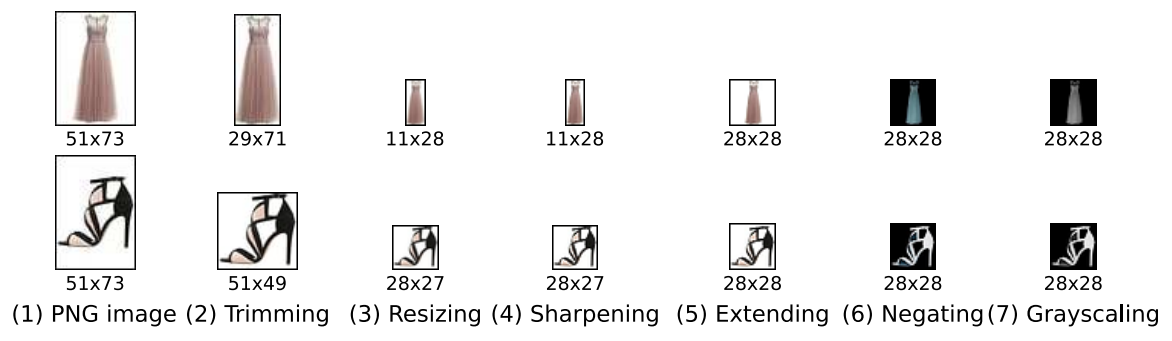
\includegraphics[width=\textwidth]{Fashion-MNIST.png}
    \caption{The conversion pipeline used to generate the \textit{Fashion-MNIST} dataset. Each row shows an example from a product category (dress, sandal), with transformations applied sequentially until the final (rightmost) image that will be part of the dataset is created.}
    \label{fig:fashion-mnist}
\end{figure*}

\textbf{Fashion-MNIST}~\cite{xiao2017fashionmnist} consists of 70,000 grayscale images of size $28\times28$, evenly distributed across 10 fashion categories such as T-shirts, trousers, coats, and shoes. The training set contains 60,000 images, and the test set includes 10,000 images. As such, the dataset is similar in structure to the MNIST digits dataset, from where it gets its name. Fashion-MNIST poses a significantly harder classification challenge: typical models that achieve over 99.7\% accuracy on digits reach only around 89–90\% on Fashion-MNIST.\\



























\begin{figure*}[t]
    \centering
    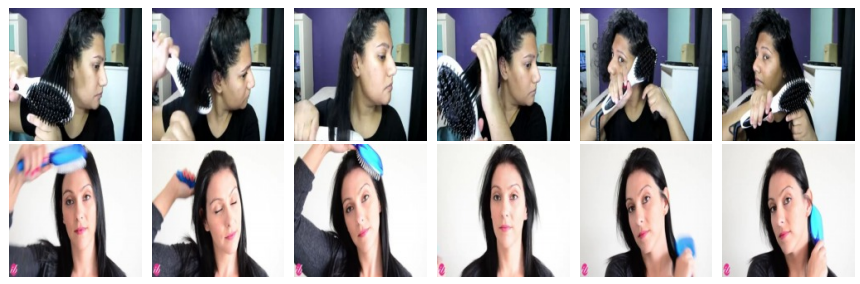
\includegraphics[width=\textwidth]{KHAVD.png}
    \caption{Example frames from the ``brushing hair'' class in the \textbf{Kinetics Human Action Video Dataset}, illustrating variation in appearance, lighting, and camera viewpoint. Each clip corresponds to a unique YouTube video.}
    \label{fig:kinetics-brushing}
\end{figure*}

The \textbf{Kinetics Human Action Video Dataset} consists of 400 action classes with approximately 400–1150 ten-second clips per class, each extracted from a distinct YouTube video (for a total of $\sim$306K clips). Actions span three major categories: \emph{person-only actions} (e.g., laughing, brushing hair), \emph{person–object interactions} (e.g., playing instruments), and \emph{person–person interactions} (e.g., shaking hands). Clips retain audio but are designed for visual classification, enabling use in multimodal learning tasks. The dataset is divided into three subsets with 250–1000 training clips per class, 50 validation clips per class, and 100 test clips per class.\\






























\begin{figure}[H]
    \centering
    \vspace{-10pt}
    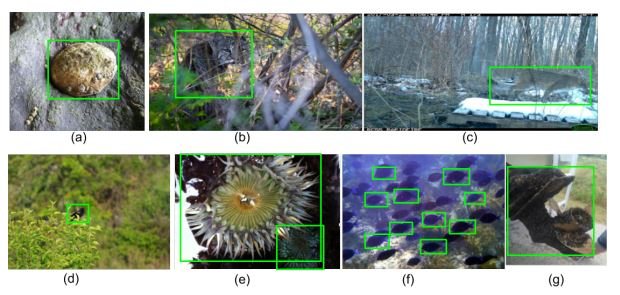
\includegraphics[width=0.5\textwidth]{iNaturalist.JPG}
    \caption{Sample bounding-box annotations for the \textbf{iNaturalist} dataset. Annotators drew boxes for the \emph{super-class} (e.g., “box all birds”), up to ten instances per image; boxes could overlap, cover only visible parts when occluded, and a single box could enclose physically connected instances.}
    \label{fig:inat2017-fig3}
    \vspace{-10pt}
\end{figure}

\textbf{iNaturalist (2017)}~\cite{vanhorn2018inaturalist}, at time of publication, contained 859,000 images (579,184 train, 95,986 val, and 182,707 test images) spanning 5,089 plant and animal species. Labels reflect the consensus of informed contributors on the iNaturalist platform, and annotators drew boxes around the plant/animals that appear on the image. On classes with the most training examples, the best classifiers at the time could only reach 67\% accuracy.\\


















\begin{figure*}[t]
    \centering
    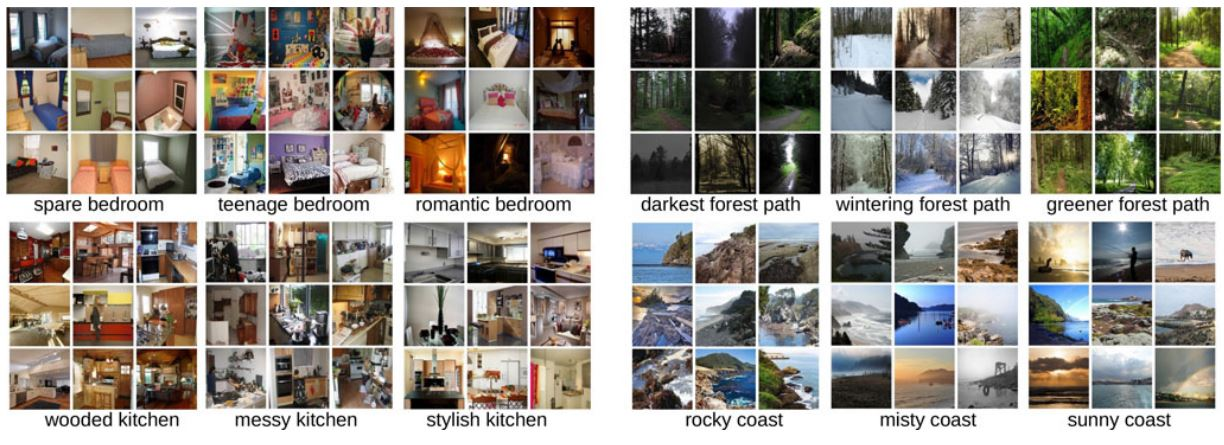
\includegraphics[width=\textwidth]{places.JPG}
    \caption{Example scenes from the \textit{Places} dataset, illustrating variations across categories such as bedrooms, kitchens, forests, and coasts. Each scene combines structural and stylistic diversity captured through adjective-based search expansions.}
    \label{fig:places}
\end{figure*}

The \textbf{Places} database~\cite{zhou2017places} comprises 10 million images labeled with 434 semantic scene categories (e.g., "messy kitchen", "misty coast"). Designed to complement object-centric datasets like ImageNet, it provides exhaustive coverage of environments such as \textit{beaches}, \textit{corridors}, \textit{kitchens}, and \textit{forests}, enabling models to understand not just objects, but the broader spatial and functional context in which they appear. An unusual and creative element of the collection process was the use of 696 English adjectives to diversify visual queries — combinations such as “messy kitchen,” “romantic bedroom,” and “misty coast.”


















\begin{figure}[H]
    \centering
    \vspace{-10pt}
    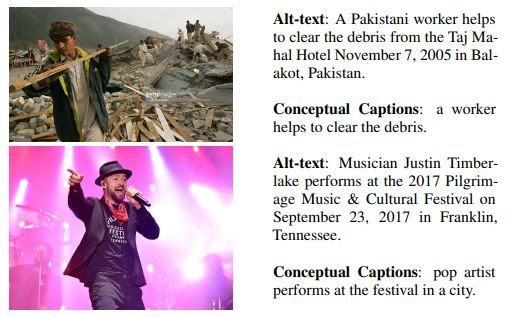
\includegraphics[width=0.5\textwidth]{ConceptualCaptions.JPG}
    \caption{Examples from the \textbf{Conceptual Captions} dataset. Original web \texttt{alt}-texts (top) are automatically cleaned and hypernymed into concise captions (bottom).}
    \label{fig:conceptual-captions}
    \vspace{-10pt}
\end{figure}

The \textbf{Conceptual Captions} dataset~\cite{sharma2018conceptual} contains about 3.3 million image–caption pairs automatically harvested from web \texttt{alt}-texts, making it over ten times larger than \textbf{MS COCO}. The final split includes 3.3 million training examples, 28,000 validation, and 22,500 test pairs, with captions averaging ten words in length. 

The dataset was created through a multi-stage automatic pipeline that processed billions of webpages. The first stage filtered out non-JPEG, small, distorted, or offensive images. In the second stage, noisy or incomplete \texttt{alt}-texts—such as keyword spam or hashtag lists—were discarded using part-of-speech, sentiment, and profanity analysis. Next, candidate captions were retained only if there was lexical overlap between concepts detected in the image (via Google Vision labels) and in the text. Finally, named entities, locations, and dates were replaced with hypernyms (e.g., “Harrison Ford” replaced by “actor”) to improve generalization. Human evaluation showed that over 90\% of captions were judged as good. 























\begin{figure*}[t]
    \centering
    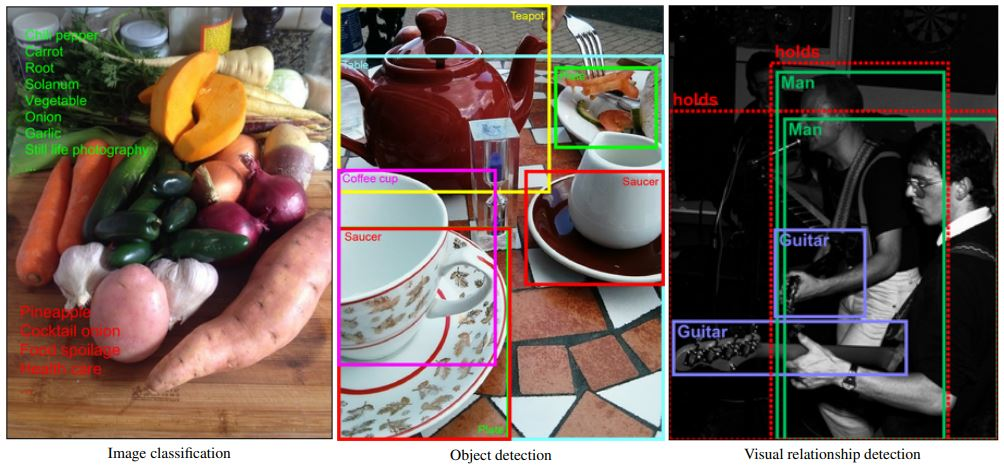
\includegraphics[width=\textwidth]{OpenImagesV4.JPG}
    \caption{Example annotations from the \textit{Open Images V4} dataset for image classification, object detection, and visual relationship detection. Green labels mark present classes, red labels absent ones. Dashed boxes group pairs of objects sharing a visual relationship.}
    \label{fig:openimages}
\end{figure*}

The \textbf{Open Images V4} dataset~\cite{kuznetsova2020openimages} contains 9.2 million Creative Commons–licensed Flickr images with unified annotations for image classification, object detection, and visual relationship detection (see Figure~\ref{fig:openimages}). It is split into 9.0M training, 41K validation, and 125K test images. It provides 30.1 million image-level labels for 19.8k concepts, 15.4 million bounding boxes for 600 object classes, and 375k relationship annotations involving 57 classes. Each image contains on average eight annotated objects, reflecting the complexity of real-world scenes.

Compared to previous datasets such as MS-COCO or ImageNet, Open Images V4 offers more than 15 times as many bounding boxes and integrates multiple annotation types within the same images.\\




































\begin{figure}[H]
    \centering
    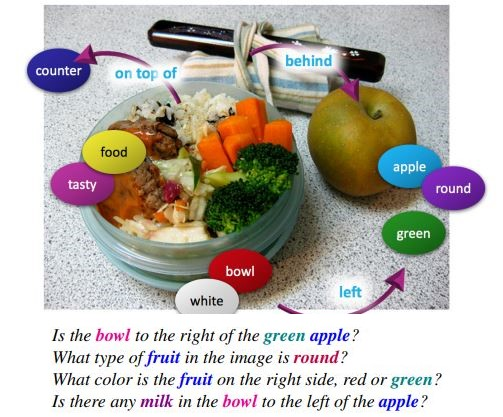
\includegraphics[width=.5\textwidth]{GQA.JPG}
    \caption{Example GQA images and queries illustrating spatial reasoning, attributes, and compositional question answering.}
    \label{fig:gqa}
\end{figure}

The \textbf{GQA} dataset~\cite{hudson2019gqa} is built upon the \textbf{Visual Genome} scene graphs and contains 113k images with 22 million automatically generated yet semantically grounded questions, of which 1.7 million form a balanced training and evaluation split. Each question is associated with a \textit{functional program} (a symbolic representation of its reasoning steps such as \texttt{select$\rightarrow$filter$\rightarrow$relate$\rightarrow$query}) and with visual justifications linking words to specific image regions.

A distinctive feature of GQA is its emphasis on compositionality: a single question may reference nested visual relationships such as “the apple on the table to the left of the bowl.” Human performance reaches 89.3\%, while strong VQA systems achieve only around 54.1\%, and a blind LSTM just 42.1\%, illustrating the task’s difficulty and the gap between recognition and reasoning. As the authors aptly remark, “It takes more than a smart guess to answer a good question,” encapsulating the spirit of the GQA benchmark.

























\begin{figure}[H]
    \centering
    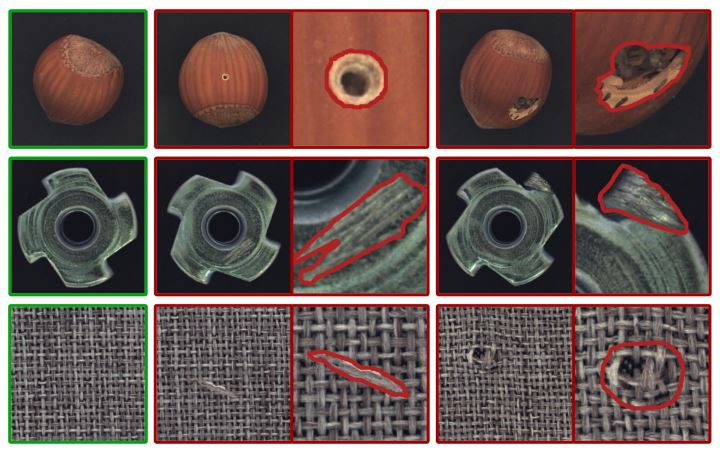
\includegraphics[width=.5\textwidth]{MVTec AD.JPG}
    \caption{Examples from \textbf{MVTec AD}: each triplet shows a defect-free image (left), an anomalous image (middle), and the pixel-precise ground-truth mask overlaid on a zoomed region (right).}
    \label{fig:mvtec-ad}
\end{figure}

The \textbf{MVTec Anomaly Detection (MVTec AD)} dataset~\cite{bergmann2019mvtec}, created by the MVTec company, attempst to solve the issue that other datasets contain only normal (defect-free) imagery is available for training. It contains 5,354 high-resolution RGB/grayscale images spanning 15 categories (10 objects and 5 textures). Training splits comprise only normal images (3,629 total), while the test split (1,725 images) mixes normal and defective cases. Anomalies cover more than 73 defect types (e.g., scratches, dents, contaminations, missing parts, and structural deformations) and every defective image is annotated with pixel-accurate ground-truth regions (1,888 masks). Images were captured with industrial telecentric optics at $\approx700\!\times\!700$–$1024\!\times\!1024$ px (this means magnification of the image does not change with the object’s distance from the lens), though some categories are grayscale only.


































\begin{figure}[H]
    \centering
    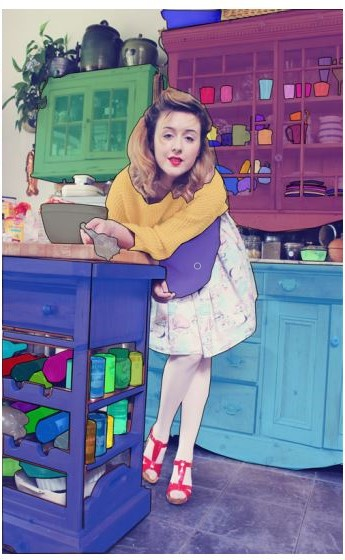
\includegraphics[width=.5\textwidth]{LVIS2.jpg}
    \caption{Example annotations from the \textbf{LVIS} dataset, illustrating fine-grained segmentation masks across diverse kitchen scenes.}
    \label{fig:lvis}
\end{figure}

The \textbf{LVIS} dataset~\cite{gupta2019lvis} (\textit{Large Vocabulary Instance Segmentation}) introduces over 1,000 entry-level object categories and aims to collect approximately two million high-quality segmentation masks over 164,000 images. Built with an “evaluation-first” philosophy, LVIS retains compatibility with the COCO average precision (AP) metric but dramatically increases category diversity while embracing the natural long-tailed distribution of real-world objects.

Unlike previous benchmarks, which exhaustively annotate a fixed set of categories, LVIS adopts a \textit{federated} dataset design. Each category has its own positive and negative subsets of images that are exhaustively annotated for that specific class, avoiding the impractical burden of labeling every image with all categories. This federated approach ensures fairness during evaluation even when an object can belong to multiple overlapping or synonymous categories. As the authors explain, “a toy deer is both a toy and a deer,” and the benchmark must fairly credit detectors that output either or both labels. Notably, LVIS segments were found to have higher boundary accuracy and annotator consistency than COCO and ADE20K masks, achieving over 99\% acceptance after verification.






































\begin{figure}[H]
  \centering
  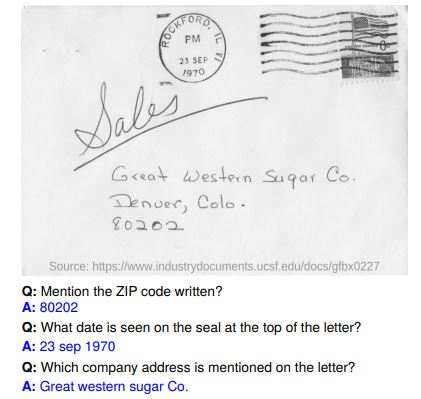
\includegraphics[width=0.5\textwidth]{DocVQA.JPG}
  \caption{\textbf{DocVQA example.} Sample document image with Q\&A pairs that require reading text and interpreting page layout/structure.}
  \label{fig:docvqa}
\end{figure}


\textbf{DocVQA}~\cite{mathew2020docvqa} is a large-scale dataset for \emph{visual question answering on document images}. It targets purpose-driven understanding of real documents (letters, forms, tables, lists, figures, and handwritten notes) to train systems that must both \emph{read} text and \emph{reason} over layout and structure. The dataset contains \textbf{12{,}767} pages drawn from \textbf{6{,}071} industry documents (spanning early 1900s–2018 and multiple domains) and \textbf{50{,}000} natural-language questions with one or more extractive answers.


Questions are answerable by copying spans \emph{verbatim} from the page (an extractive QA setting). Success therefore couples robust OCR with structural understanding: models must leverage cues like headings, seals, key–value pairs, table cells, and relative position (e.g. “at the top left”, “in the seal”, “ZIP code”). Data are split \textbf{80/10/10} into train/val/test: 39,463/5,349/5,188 questions over 10,194/1,286/1,287 images. Human accuracy is reported at \textbf{94.36\%}, leaving a substantial gap for current VQA/MRC baselines that struggle especially on structure-heavy queries.





















\begin{figure*}[t]
    \centering
    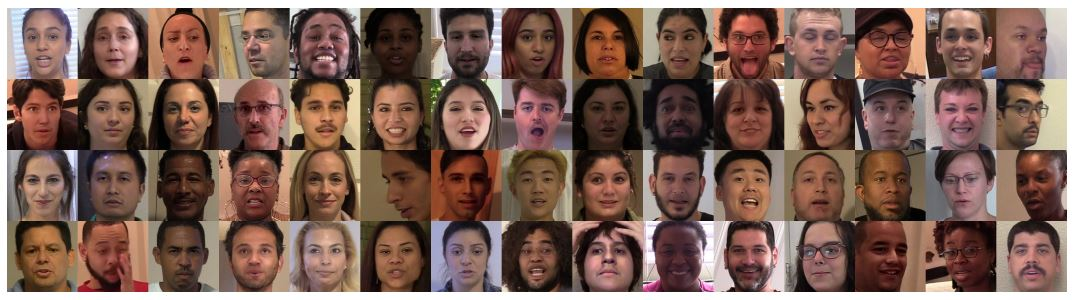
\includegraphics[width=\textwidth]{DFDC.JPG}
    \caption{\textbf{DFDC face mosaic.} Example frames from the DFDC dataset. All identities are consenting paid actors recorded specifically for creating and detecting face swaps.}
    \label{fig:dfdc}
\end{figure*}

The \textbf{DeepFake Detection Challenge (DFDC)} dataset~\cite{dolhansky2020dfdc} is a large, consented face-swap corpus designed for training and benchmarking Deepfake detectors. It comprises 100k+ 10-second clips sourced from 3,426 paid actors (average 14.4 videos/subject; mostly 1080p), totaling 38.4 days of footage and 25TB of raw data. Relative to previous datasets, DFDC is orders-of-magnitude larger, higher quality, and ethically collected with explicit consent.

Multiple techniques (Deepfake Autoencoder, morphable-mask, Neural Talking Heads, and so on) were used to make the fake videos so that detection models wouldn’t just overfit to one kind of fake, but would learn to generalize to many.\\




































\begin{figure*}[t]
    \centering
    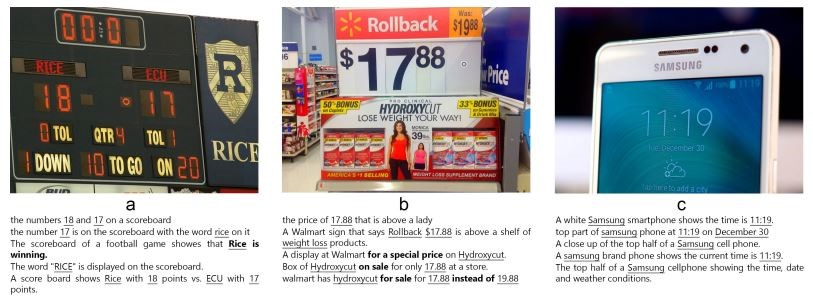
\includegraphics[width=\textwidth]{TextCaps3.jpg}
    \caption{Examples from TextCaps demonstrating how captions combine visual description with textual information in the image. Bold phrases indicate paraphrasing or reasoning; underlined ones are directly copied OCR text.}
    \label{fig:textcaps2}
\end{figure*}

The \textbf{TextCaps} dataset~\cite{sidorov2020textcaps} introduces the task of image captioning with reading comprehension, where models must both recognize scene text and reason about it within the visual context. For example, recognizing a “red sign” is insufficient, the model must read “Mornington Crescent” to identify the location, or understand that “Rice is winning” implies interpreting a scoreboard rather than simply detecting numbers. The dataset contains 145,000 captions over 28,000 images belonging originally to OpenImages v3.























\begin{figure*}[t]
    \centering
    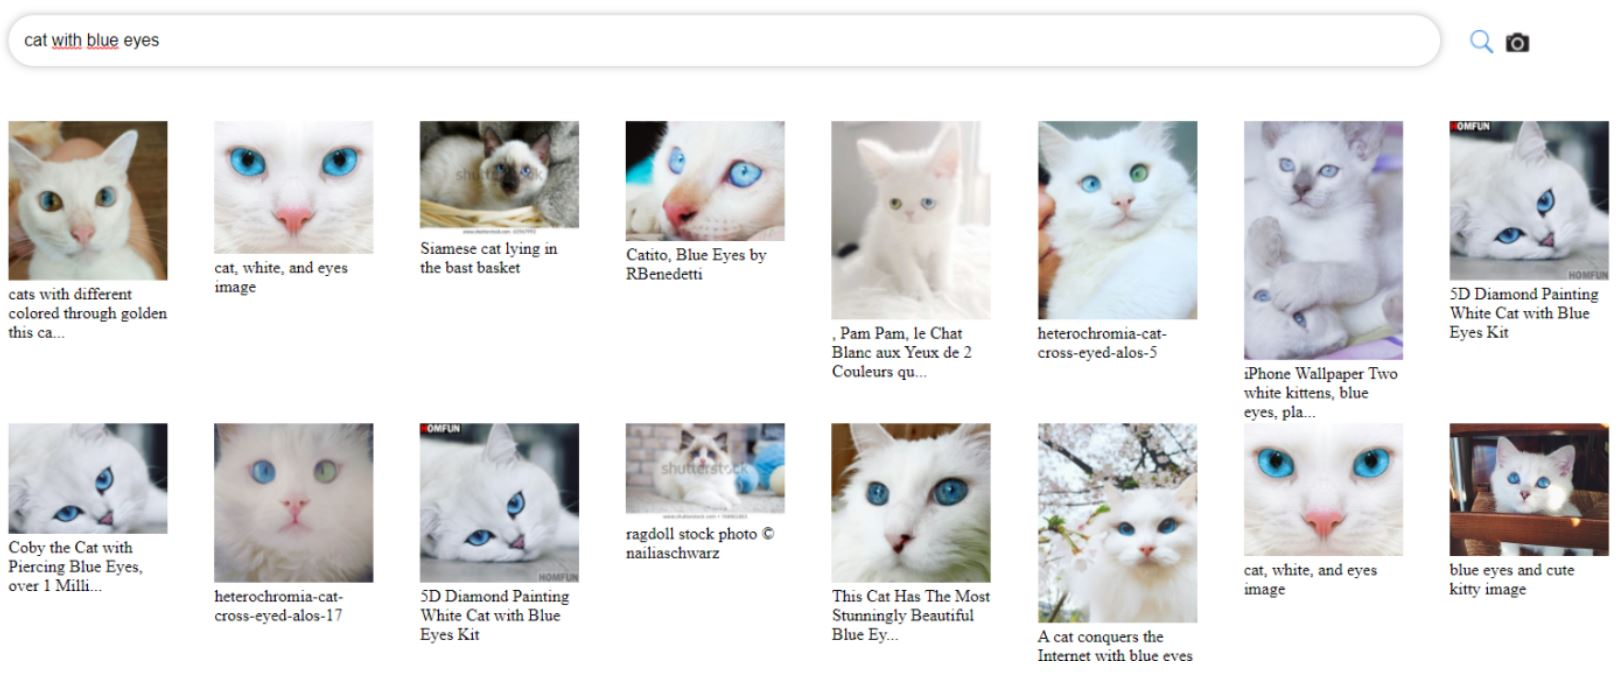
\includegraphics[width=\textwidth]{LAION-400M.JPG}
    \caption{Example image retrieval results for the query ``cat with blue eyes'' using the LAION-400M web demo. The dataset supports large-scale multimodal similarity search using CLIP embeddings.}
    \label{fig:laion400m}
\end{figure*}

The \textbf{LAION-400M} dataset~\cite{schuhmann2021laion400m} contains an astounding 400 million image–text pairs, filtered using \textbf{CLIP} to ensure semantic alignment between images and captions. It was created as a community-driven effort to provide a large-scale, public alternative to proprietary datasets used to train models such as CLIP and DALL·E. Each entry includes an image URL, text caption, CLIP embeddings for both modalities, metadata (license type, image size, and NSFW tag), and precomputed kNN indices for efficient similarity search. 




















\begin{figure*}[t]
    \centering
    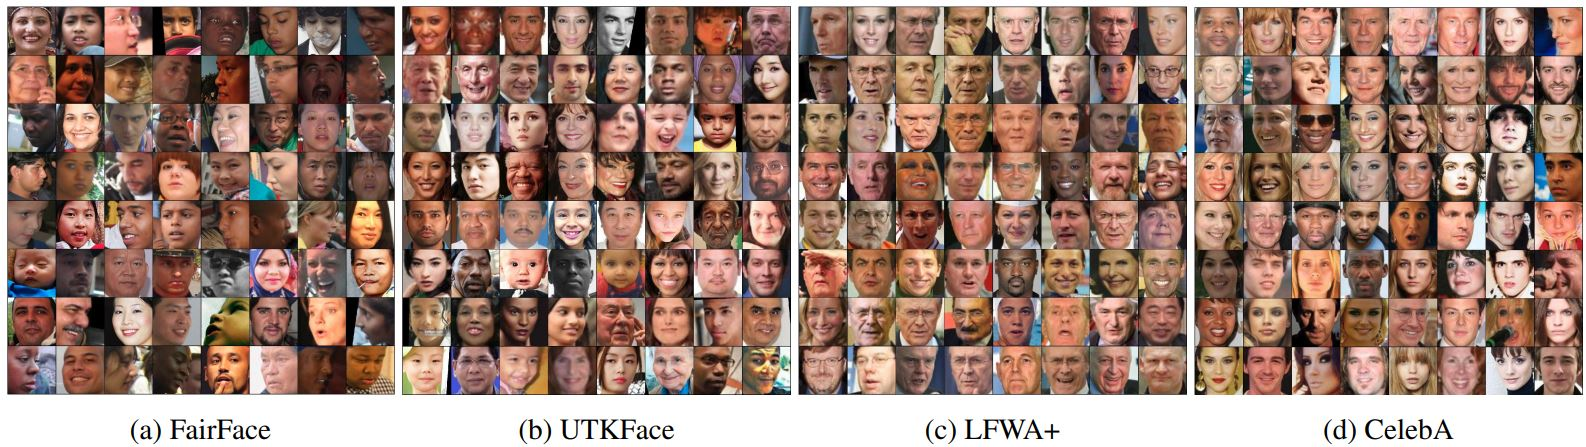
\includegraphics[width=\textwidth]{FairFace.JPG}
    \caption{Example faces from (a) FairFace and (b–d) popular prior datasets. FairFace is designed to be racially balanced, unlike many existing sets that are dominated by White faces.}
    \label{fig:fairface_grid}
\end{figure*}

\textbf{FairFace}~\cite{karkkainen2021fairface} introduces 108,501 in-the-wild face images with labels for race, gender, and age, constructed to be balanced over seven race groups: White, Black, Indian, East Asian, Southeast Asian, Middle Eastern, and Latino, which were annotated manually. 

The paper highlights that many widely used face datasets (e.g., celebrity or politician collections) are skewed toward lighter-skin/White faces, which leads to uneven accuracy across demographics. Models trained on FairFace yield higher and more consistent accuracy across race and gender on these novel sets, even when FairFace’s training subset is down-sampled. 
























\begin{figure}[H]
    \centering
    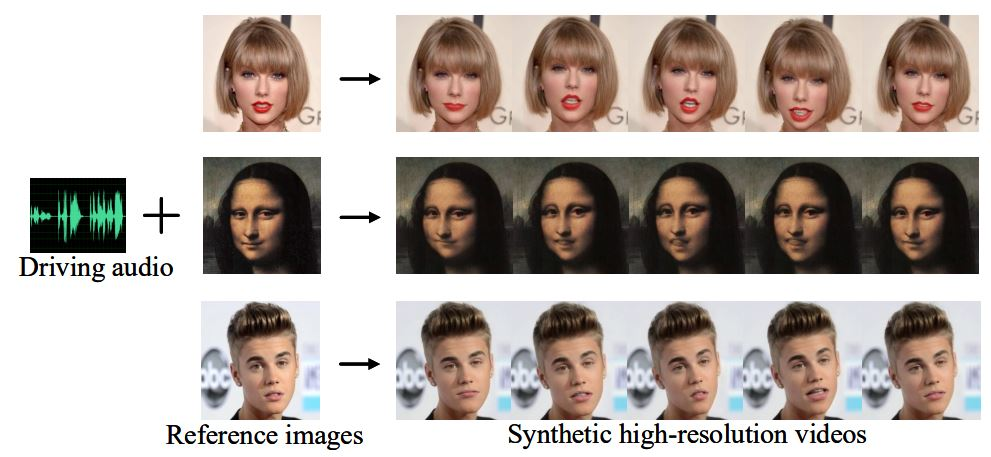
\includegraphics[width=0.5\textwidth]{HDTF.JPG}
    \caption{Overview of one-shot high-resolution talking face generation from the HDTF dataset. Given a reference image and driving audio, the model synthesizes high-resolution videos with synchronized facial animation.}
    \label{fig:hdtf}
\end{figure}

\noindent
\textbf{HDTF}~\cite{zhang2021hdtf} authors note that prior systems top out around 256$\times$256, so that they introduce High-Definition Talking Face (HDTF), a high-definition, in-the-wild dataset ($\sim$16 hours of 720p--1080p video, 300+ subjects, 10k+ sentences) curated from recent YouTube content so the crops remain sharp after 512$\times$512 resizing. They synthesize high-definition, lip-synchronous videos (demonstrations include portraits and paintings) and report both objective and user-study gains over landmark-based baselines, especially at $512\times 512$.
































\begin{figure*}[H]
    \centering
    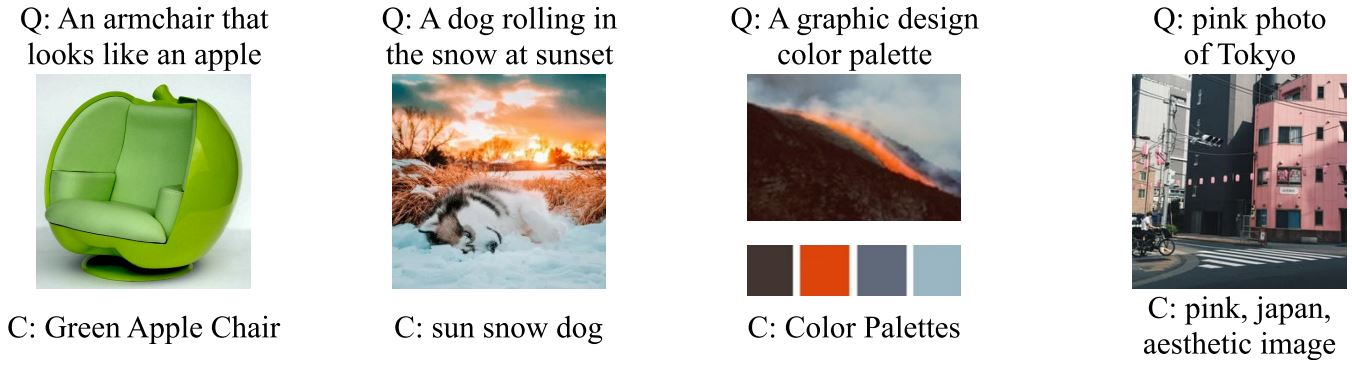
\includegraphics[width=\textwidth]{LAION-5B.JPG}
    \caption{Nearest-neighbor examples from LAION-5B using CLIP embeddings. For each text query (Q), the corresponding top retrieved image and its caption (C) are shown.}
\end{figure*}

The LAION-5B dataset~\cite{schuhmann2022laion5b} is the largest openly available image–text dataset ever released, designed to democratize research on large-scale multimodal models such as \textbf{CLIP}, \textbf{GLIDE}, and \textbf{Stable Diffusion}. It contains 5.85 billion CLIP-filtered image–text pairs collected from Common Crawl, including 2.32 billion English pairs, 2.26 billion multilingual pairs covering over a hundred languages, and 1.27 billion language-agnostic samples, which often describe products or places. Each entry is accompanied by metadata such as the image URL, caption text, image dimensions, cosine similarity between the image and text embeddings, and safety-related scores like watermark and NSFW probabilities.

The accompanying web interface allows interactive dataset exploration, nearest-neighbor search via CLIP embeddings, and flexible subset generation. The dataset has been validated through extensive experiments. Models trained on \textbf{LAION-400M} reproduce the zero-shot classification performance of OpenAI’s CLIP on ImageNet and other benchmarks, confirming that the filtering and scale of LAION-5B provide data of comparable quality. Subsets such as LAION-Aesthetics and LAION-High-Resolution have also been derived to train models like Stable Diffusion, which achieve state-of-the-art results in text-to-image generation. 
























\begin{figure}[H]
    \centering
    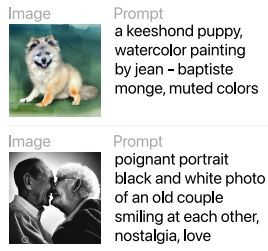
\includegraphics[width=0.35\textwidth]{DiffusionDB2.jpg}
    \caption{Examples from \textbf{DiffusionDB}, showing generated images with their corresponding prompts}
    \label{fig:diffusiondb}
\end{figure}

\noindent
\textbf{DiffusionDB}~\cite{wang2022diffusiondb} is the first large-scale, community-generated prompt dataset for text-to-image diffusion models. It contains over 14 million images, 1.8 million unique text prompts, and detailed \textbf{Stable Diffusion hyperparameters} including seed, step count, CFG scale, sampler type, image size, and timestamp. The dataset was collected from the official Stable Diffusion public Discord server, where users shared their generation results. To ensure safe and ethical use, the authors applied state-of-the-art NSFW detection models on both images and prompts, producing continuous safety scores that allow flexible filtering. Prompts were also analyzed linguistically and semantically: most are short (6–12 tokens) and in English, but the dataset spans over 30 languages.\\



















































\begin{figure}[H]
  \centering
  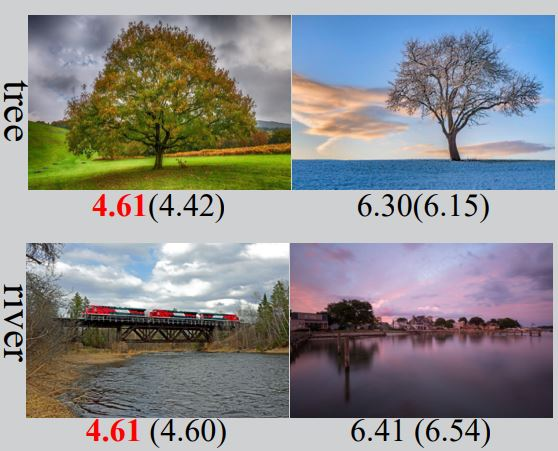
\includegraphics[width=0.45\textwidth]{TAD66K.JPG}
  \caption{Examples from the \textbf{TAD66K} dataset~\cite{he2022tad66k}. Each pair shows images from the same theme with their average aesthetic scores (in red) and predicted scores in parentheses. Even when scores are similar, different themes correspond to distinct aesthetic criteria.}
\end{figure}

The \textbf{TAD66K} dataset~\cite{he2022tad66k} (Theme and Aesthetics Dataset) was created to address a key issue in image aesthetics assessment (IAA): different image themes follow distinct evaluation criteria, yet existing datasets and models generally ignore this fact. TAD66K contains approximately 66,327 carefully curated images covering 47 popular themes, organized into seven super-themes (plants, animals, artifacts, colors, humans, landscapes, and others). Each image was selected manually to ensure thematic clarity and diversity. Every image is annotated with an aesthetic score from 1 to 10, and unlike previous datasets that measure aesthetics, TAD66K provides theme-specific evaluation criteria. For instance, the aesthetic standards applied to images of trees differ from those for rivers or people. 












































\begin{figure*}[t]
  \centering
  % Replace the filename below with your local path if needed
  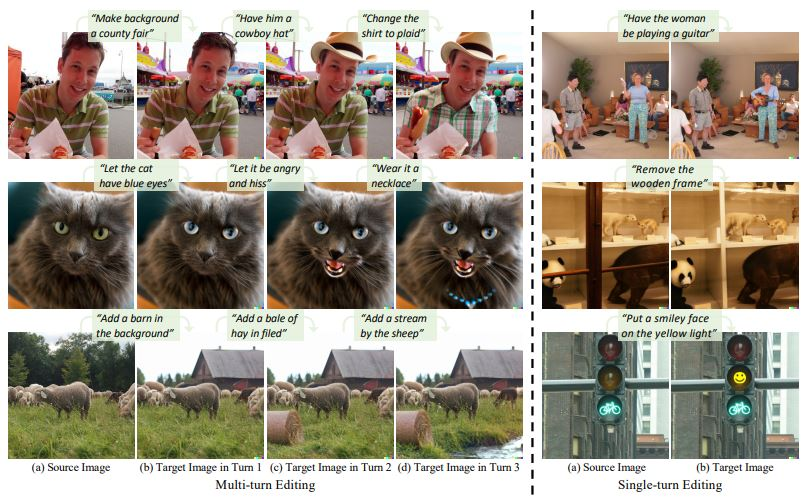
\includegraphics[width=\linewidth]{MagicBrush.JPG}
  \caption{Illustration of \textsc{MagicBrush}: instruction–guided real image editing with both \emph{multi–turn} (left) and \emph{single–turn} (right) workflows. Each triplet consists of a source image, a natural–language instruction, and a target image.}
  \label{fig:magicbrush}
\end{figure*}


\textbf{MagicBrush}~\cite{zhang2023magicbrush} is a manually annotated dataset for instruction–guided real image editing. It contains 5,313 edit sessions and 10,388 turns (~10K triplets: source image from MS COCO, instruction, target image). Images are modified with DALL·E~2 until an instruction-consistent, photorealistic target was obtained. As shown in Figure~\ref{fig:magicbrush} some sessions are single-turn, others are multi-turn. 










































\begin{figure}[H]
    \centering
    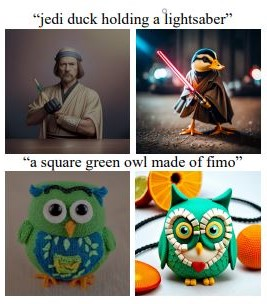
\includegraphics[width=0.35\textwidth]{PickAPic2.jpg}
    \caption{\textbf{Pick-a-Pic} web-app outputs. For each prompt the non-preferred image (left) is darkened and the user-preferred image (right) is highlighted.}
    \label{fig:pickapic2}
\end{figure}

\textbf{Pick-a-Pic}~\cite{kirstain2023pickapic} is a dataset of human preferences for text-to-image generation, collected through a public web application in which users write prompts, generate images with modern diffusion models, and select which image they prefer (or declare a tie). Each datapoint contains a prompt, two model outputs, and a preference label. The initial release contains over $\sim$ 500K pairwise judgments drawn from $\sim$ 35K prompts (and continues to grow), with images produced by Stable Diffusion~2.1, Dreamlike Photoreal~2.0, and SDXL variants under multiple classifier-free guidance (CFG) scales. 


















\begin{figure*}[t]
    \centering
    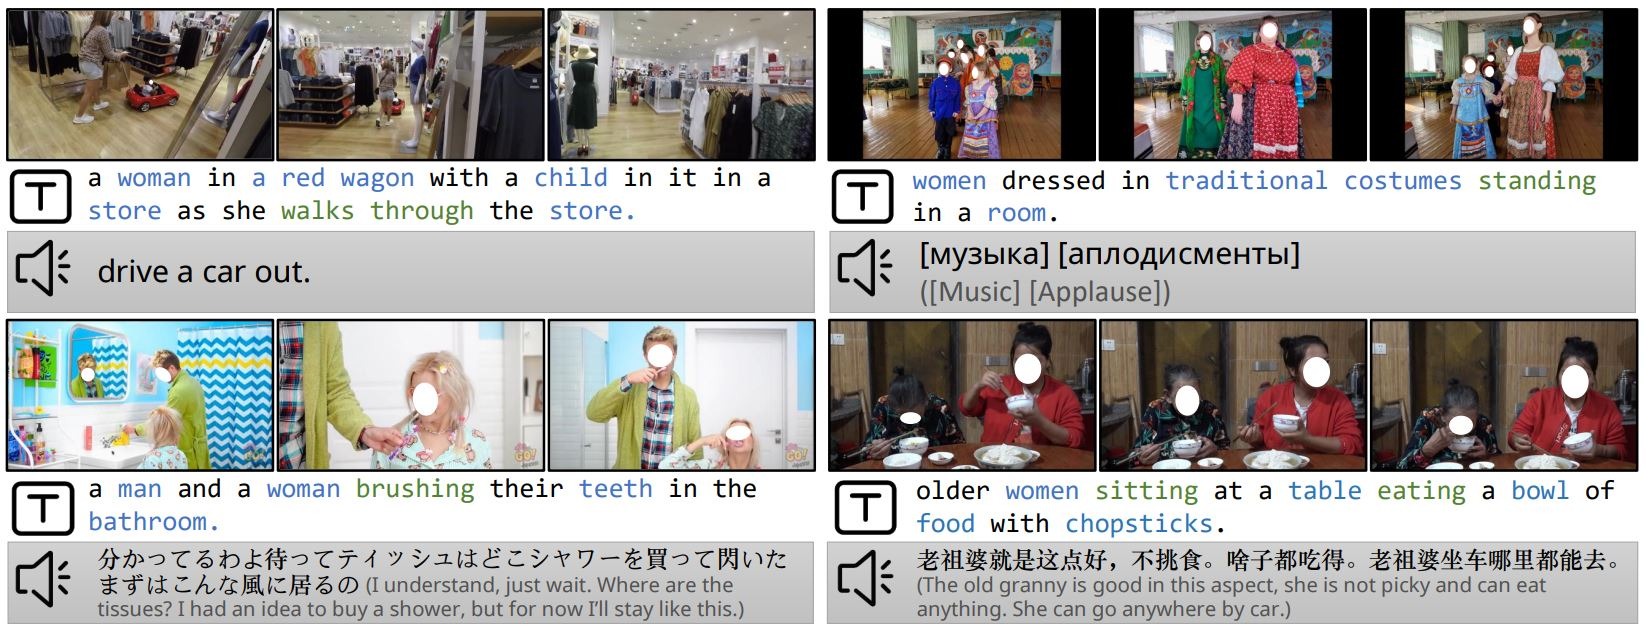
\includegraphics[width=\textwidth]{InternVid.JPG}
    \caption{Examples from \textbf{InternVid}. For each video clip (three frames shown), the dataset provides LLM-generated captions that emphasize nouns (blue) and verbs (green). Compared with raw ASR transcripts (grey), the captions are more visually grounded and descriptive.}
\end{figure*}

\textbf{InternVid}~\cite{wang2023internvid} comprises \textasciitilde7.1M public YouTube videos spanning \textasciitilde760K hours and yields \textasciitilde234M trimmed clips (median \textasciitilde10\,s) paired with \textasciitilde4.1B caption words. Coverage is intentionally broad: 16 topical domains, \textasciitilde6,100 action phrases used as queries, and geographically diverse sources; \textasciitilde85\% of videos are 720p (remainder 360–512p). 
































\begin{figure*}[t]
    \centering
    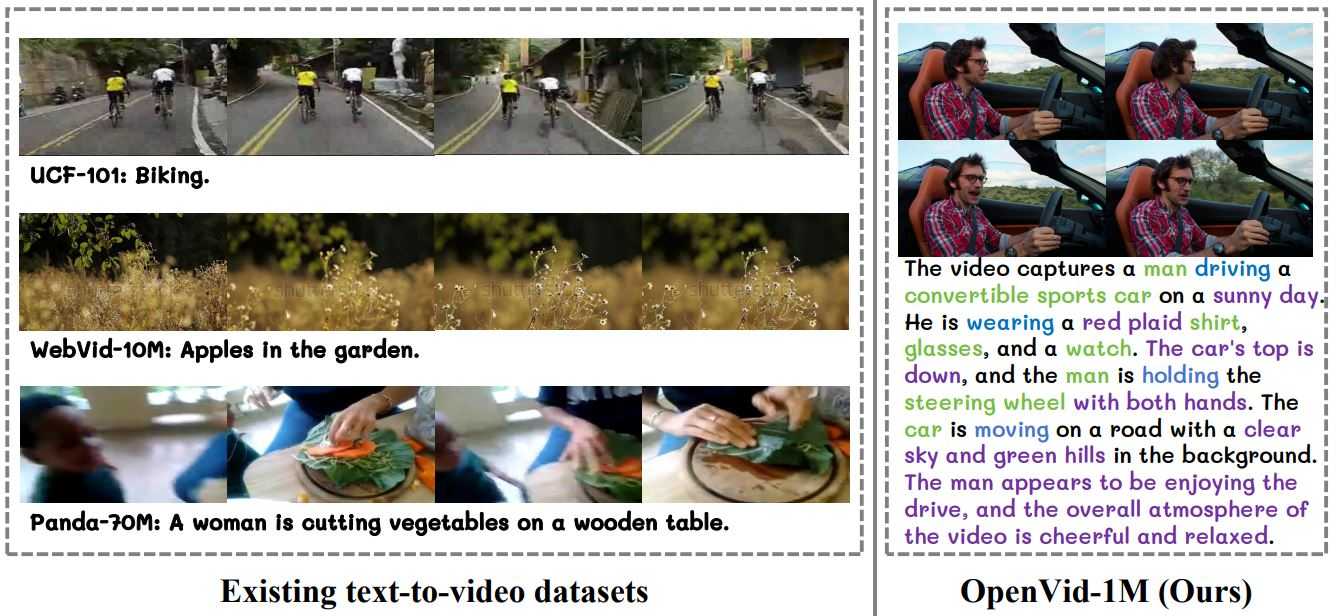
\includegraphics[width=\textwidth]{OpenVid-1M.JPG}
    \caption{Comparison between existing text-to-video datasets and OpenVid-1M. Datasets such as UCF-101, WebVid-10M, and Panda-70M often contain low-resolution or low-quality videos with short captions, whereas OpenVid-1M features over one million high-quality clips with expressive, detailed textual descriptions highlighting both semantic and visual nuances.}
    \label{fig:openvid1m}
\end{figure*}

\textbf{OpenVid-1M}~\cite{nan2024openvid} is a large-scale open-scenario dataset containing over one million high-quality text–video pairs, each accompanied by very descriptive captions, as shown in Figure~\ref{fig:openvid1m}. Prior datasets such as WebVid-10M and Panda-70M prioritize size over fidelity and contain numerous low-resolution, watermarked, flickering, or blurry videos, such is the issue OpenVid-1M seeks to solve. 

The dataset was built by processing large collections such as Panda-50M, ChronoMagic, CelebV-HQ, and Open-Sora-Plan. Videos were evaluated according to multiple criteria, such as using the LAION Aesthetics Predictor to retain only the top 20\% of visually appealing clips. The rather descriptive captions were then generated or rewritten via the multimodal model LLaVA-v1.6-34B.

To further advance high-definition video generation, 433K of these clips at 1080p resolution were selected to create OpenVidHD-0.4M. Overall, OpenVid-1M comprises 1,019,957 clips averaging 7.2 seconds each (approximately 2,051 total hours of content), all at least $512\times512$ in resolution. 

Experimental results confirm that OpenVid-1M and MVDiT significantly outperform prior approaches. Models trained on OpenVid-1M achieve higher aesthetic (VQAA) and technical (VQAT) scores, improved text–video alignment (SD\_score and Blip\_BLEU), and better temporal coherence (Clip\_temp\_score). \\































\begin{figure*}[t]
  \centering
  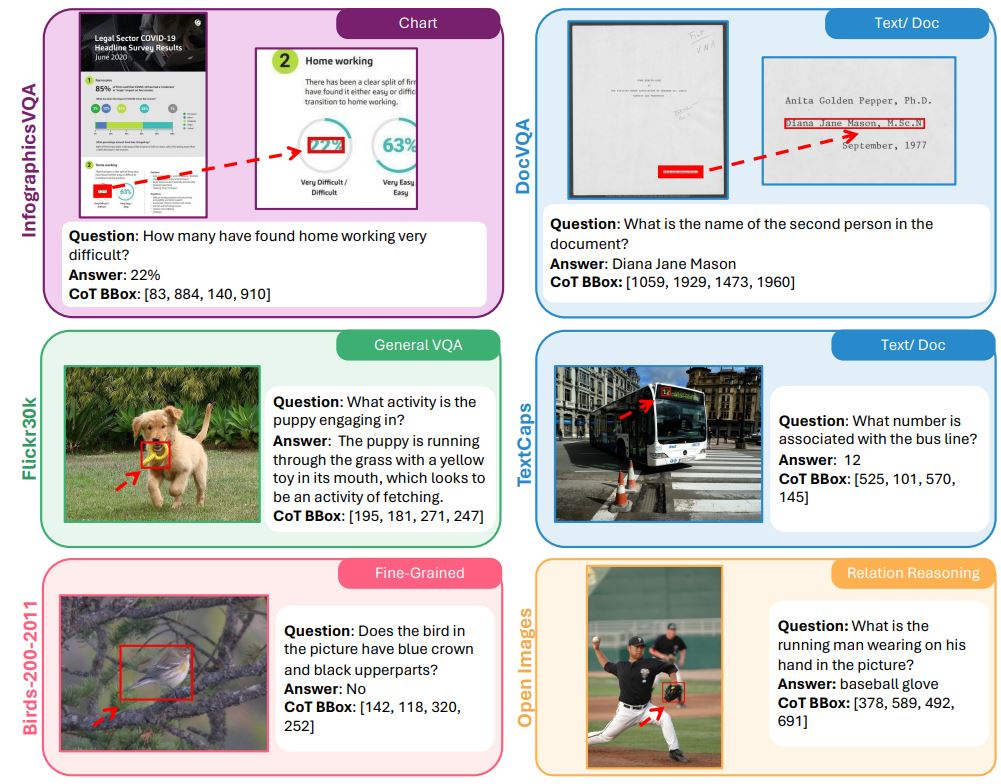
\includegraphics[width=\textwidth]{Visual CoT.JPG}
  \caption{\textbf{Visual CoT} examples across five domains. Each question–answer pair is accompanied by an intermediate bounding box (red) that highlights the key region used in reasoning.}
\end{figure*}

\textbf{Visual CoT}~\cite{shao2024visualcot} contains 438K question–answer pairs, each annotated with a grounding bounding box that marks the critical image region required to answer the question; approximately 98K pairs additionally include step-by-step visual–textual reasoning. Data span five domains: text/doc understanding, fine-grained recognition, charts, general VQA, and relation reasoning, and are built from twelve source corpora (e.g., TextVQA, DocVQA, TextCaps, Flickr30k,GQA, Open Images). \\





























\begin{figure*}[t]
    \centering
    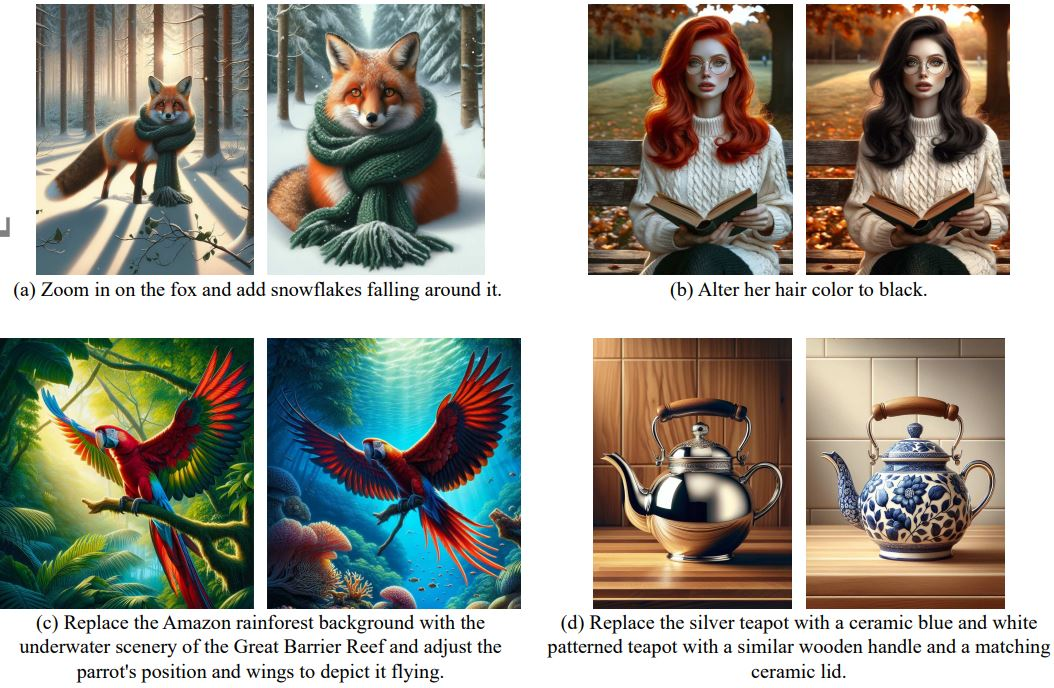
\includegraphics[width=\textwidth]{HQ-Edit.JPG}
    \caption{(a)–(d): example image edit pairs and instructions from HQ-Edit. (e): comparison of dataset quality between HQ-Edit and previous benchmarks. “Alignment” and “Coherence” are newly proposed metrics introduced in Section~3.4 to evaluate semantic and aesthetic quality.}
    \label{fig:hqedit}
\end{figure*}

\textbf{HQ-Edit}~\cite{hui2024hqedit} comprises approximately 200,000 instruction-based image edits. Unlike earlier datasets that rely on people to give feedback, HQ-Edit collects data automatically using advanced models: GPT-4V and DALL-E 3. This method creates clearer, higher-quality images and more accurate text instructions, making the link between the text and image much stronger.

In addition to automatic evaluation, a human study on 1,651 image pairs generated by DALL-E~3 was conducted to validate the proposed metrics. Participants rated how well the output images reflected the corresponding edit instructions on a five-point scale, ranging from “totally unrelated” to “perfectly aligned.” Pearson correlation analysis revealed that HQ-Edit’s Alignment metric strongly correlates with human judgments and significantly outperforms the commonly used CLIP Directional Similarity score, which often fails to capture nuanced, instruction-level edits. Furthermore, fine-tuning InstructPix2Pix on HQ-Edit results in a substantial performance boost, achieving a $12.3$-point increase in Alignment and a $5.64$-point improvement in Coherence over the vanilla model.\\













\textbf{BLIP3o-60k}~\cite{chen2025blip3o} is a 60,000-sample instruction-tuning dataset built by prompting GPT-4o with textual inputs covering various visual domains, including scenes, everyday objects, artistic styles, lighting conditions, gestures, and compositions. Each example in BLIP3o-60k consists of an instruction prompt, a corresponding image, and the image’s CLIP feature embedding. The prompts are designed to mimic real-world creative instructions, such as “a person jumping in the rain wearing a yellow coat” or “an ancient city at sunset in watercolor style”.\\





























\begin{figure*}[t]
  \centering
  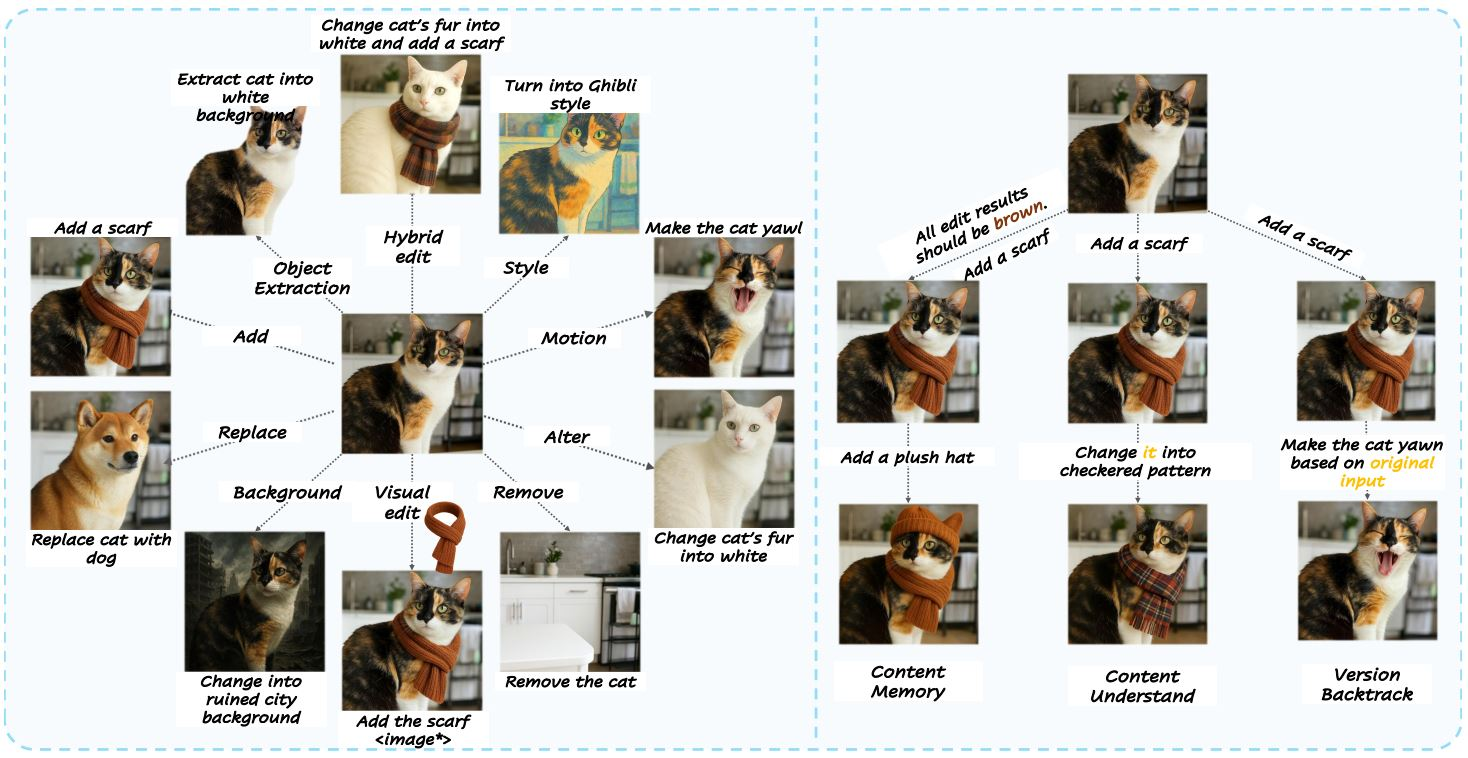
\includegraphics[width=\textwidth]{ImgEdit.JPG}
  \caption{\textbf{ImgEdit} illustrates single–turn edits (add, remove, replace, alter, background/style change, motion change, object extraction, visual and hybrid edits) and multi–turn behaviors (content memory, content understanding, version backtracking).}
\end{figure*}

The \textbf{ImgEdit} dataset~\cite{ye2025imgedit} contains 1.2M carefully curated edit pairs at high resolution (shorter side $\ge\!1280$), including 1.1M single–turn samples spanning 10 representative operations (local: add, remove, replace, alter, motion change, object extraction; global: background/style; visual edit via reference; hybrid edits that compose multiple local ops) and 110K multi–turn samples covering content memory, content understanding, and version backtracking. 

The original images come from a high–aesthetics subset of LAION (aesthetic score $>\!4.75$ and resolution filtering). These go through multiple steps to generate the edits, including: the creation of concise captions and candidate edit targets with \textbf{GPT-4o}, validation of regions to be edited by CLIPScore and area thresholds (e.g., background edits must occupy $>\!40\%$ of the image), and prompt-guided post-filtering, returning quality scores.\\


























\begin{figure*}[t]
  \centering
  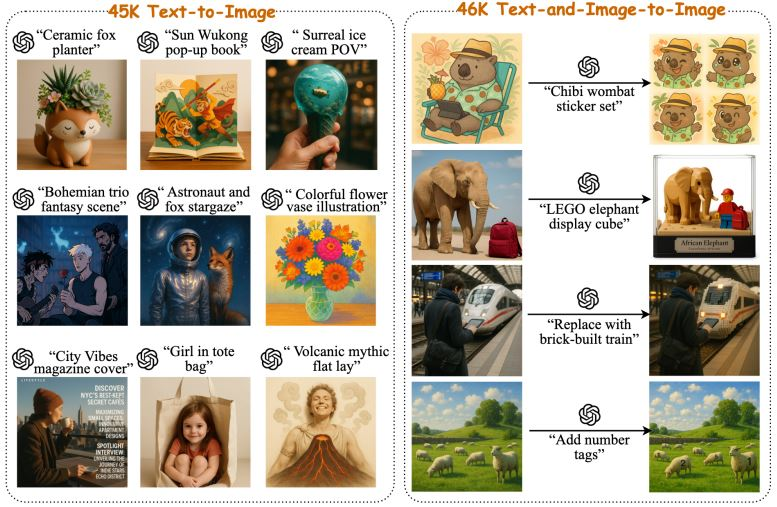
\includegraphics[width=\textwidth]{sharegpt4o.JPG}
  \caption{\textbf{ShareGPT-4o-Image}. Examples from the two splits: \emph{45K} text-to-image (left) and \emph{46K} text\&image-to-image (right) synthesized by GPT-4o-Image.}
\end{figure*}

\textbf{ShareGPT-4o-Image}~\cite{chen2025sharegpt} contains 91K synthetic samples comprising 45K text-to-image pairs and 46K instruction-guided text\&image-to-image triplets, where every target image is produced by GPT-4o-Image. The two distinct sets go through specific pipelines to arrive at the result.

\end{multicols}


\clearpage
\subsection{Benchmark Tasks and Metrics}
\label{sec:benchmark-tasks}

The execution loop is shared by every task family. As shown in
Listing~\ref{lst:benchmark-loop}, each sample is loaded, converted into a
task-specific prompt, sent to the chosen model, timed, and evaluated. Errors
are recorded as failed samples rather than terminating the complete run. This
behaviour was particularly important for long API experiments, where one
network or dataset error should not discard hours of completed work.

\begin{lstlisting}[caption={Core per-sample execution from
\texttt{benchmarks/\_base\_benchmark.py}.},label={lst:benchmark-loop}]
for idx, row in enumerate(rows, start=1):
    sample_started_at = time.perf_counter()
    try:
        image = self.get_image_for_row(row)
        prompt_labels = self.get_prompt_labels_for_row(
            row=row, labels=labels
        )
        prompt = self.make_prompt(
            labels=prompt_labels, row=row, image=image
        )
        generation_started_at = time.perf_counter()
        prediction = model.predict(image, prompt).strip()
        generation_time_seconds = (
            time.perf_counter() - generation_started_at
        )
    except Exception as exc:
        sample_error = f"{exc.__class__.__name__}: {exc}"
\end{lstlisting}
\subsubsection{\textbf{L}: Labeling}

This benchmark takes one image and a list of possible labels. The model returns exactly one label describing the image. For video datasets, several frames are combined into a contact sheet and the model predicts the action or video label.

The smallest context windows among the listed models appear to be those of
\texttt{glm-4.5v-thinking} and \texttt{glm-4.1v-thinking}, both at 64k tokens.
Depending on whether one uses the official serving configuration rather than
the Hugging Face architectural config, \texttt{dots.vlm1} may also be treated
as a 65,536-token model.

Among the classification datasets considered in this study, the largest label spaces correspond to ImageNet-1K, iNaturalist, and Open Images V4. ImageNet-1K contains 1,000 classes, iNaturalist contains 5,089 species categories, and Open Images V4 provides approximately 20,000 image-level concepts. Since all evaluated models support context windows of at least 64k input tokens, the complete label set can be provided as part of the prompt for ImageNet-1K without difficulty.

For iNaturalist, only the species-level labels will be included in the prompt. This reduces the required prompt length to approximately 20k--30k tokens while preserving the standard fine-grained classification task. Higher levels of the taxonomic hierarchy (e.g., genus, family, order, and class) will not be provided as candidate labels.

For Open Images V4, the full image-level vocabulary is too large to be comfortably included within a 64k-token context window. Therefore, only the subset of images associated with bounding-box annotations will be used. This restricts the candidate label set to the 600 object categories employed by the detection benchmark, allowing all possible labels to be supplied in the prompt while maintaining a closed-set classification setting.

\subsubsection{\textbf{A:} Answering Visual Multiple-choice Question}

This benchmark takes an image, a natural-language question about its contents, and a set of possible answers. The model selects one answer, which is normalized and compared with the accepted reference answer.

All VQA is multiple choice. For some dataset, distractor choices had to be manually created. For others, even the correct choices had to be created.

The distractor choices must be created for \textbf{Visual Genome}, \textbf{VQA v2.0}, \textbf{GQA}, \textbf{DocVQA}, and \textbf{Visual CoT}. These datasets already provide each image, question, and accepted answer, so the accepted answer can be used as the correct choice; however, their dataset adapters do not provide a set of incorrect candidate answers. Consequently, plausible but incorrect distractors must be added to convert these open-answer questions into multiple-choice questions.

\textbf{FlyingThings3D} requires more extensive construction because it is not originally a question--answer dataset. It provides rendered stereo scenes and geometric annotations rather than natural-language questions with accepted answers. For this dataset, the question and correct textual choice must first be derived from the available scene information; the incorrect choices must then also be created. Thus, only the distractors need to be added for the five existing QA datasets, whereas both the benchmark question/answer and its distractors need to be constructed for FlyingThings3D.

Visual Genome has bouding boxes, but these are very inconsitent because they are human anotatesd without a standard list of labels, so we may get `pet dog` somewhere, but `small dog` elsewhere. That is why we will not measure it in terms of boudning boxes. Moreover, there are over 30k different types of annotated objects, which would not fit into our maximum of 64k labels.

\subsubsection{\textbf{B}: Bounding Box Object Detection}

This benchmark takes an image and a list of allowed object labels. The model returns every detected object as a label and normalized bounding box. Predictions are compared with annotated boxes using label agreement and intersection over union (IoU).

Listing~\ref{lst:detection-metrics} contains the metric calculation used after
predicted and ground-truth boxes have been greedily matched at the configured
IoU threshold. Reporting precision, recall, and F1 separately is useful:
precision exposes excessive boxes, recall exposes missed objects, and F1
summarises both errors without hiding them.

\begin{lstlisting}[caption={Detection scoring from
\texttt{benchmarks/detection/\_detection.py}.},
label={lst:detection-metrics}]
matched_predictions, matched_targets, matched_ious = (
    self._match_boxes(pred_boxes, gt_boxes)
)
tp = len(matched_predictions)
fp = max(0, len(pred_boxes) - tp)
fn = max(0, len(gt_boxes) - tp)

precision = tp / (tp + fp) if (tp + fp) else 0.0
recall = tp / (tp + fn) if (tp + fn) else 0.0
f1 = (
    2 * precision * recall / (precision + recall)
    if (precision + recall) else 0.0
)
\end{lstlisting}

\subsubsection{\textbf{C}: Captioning}

This benchmark takes an image, or representative frames from a video, without answer choices. The model generates one concise natural-language description. It is compared with one or more reference captions using BLEU.

The caption evaluator in Listing~\ref{lst:caption-metric} uses the same
references exposed by the dataset adapter and records the continuous BLEU
score even when the binary threshold is not reached. This is why the report
can compare mean caption quality without reducing every answer to only correct
or incorrect.

\begin{lstlisting}[caption={Caption evaluation from
\texttt{benchmarks/captioning/\_captioning.py}.},
label={lst:caption-metric}]
references = self._get_captions(row)
bleu = self._sentence_bleu(
    references=references,
    candidate=prediction,
)
return (
    bleu >= self.bleu_threshold,
    references,
    {
        "bleu": bleu,
        "reference_captions": references,
    },
)
\end{lstlisting}

\subsubsection{\textbf{E}: Editing Prompt Reconstruction}

This benchmark takes a side-by-side pair containing the original image and its edited version, plus four candidate editing prompts. The model selects the prompt that best explains the transformation from the first image to the second.

\subsubsection{\textbf{G}: Generating Prompt Reconstruction}

This benchmark takes an image generated from text and four candidate generation prompts. The model selects the prompt that most likely produced the image, returning either its choice letter or the exact prompt.

\subsubsection{\textbf{P}: Preference}

This benchmark takes two images shown side by side. The model chooses which image is preferred by returning Image A or Image B. The choice is compared with the recorded human preference.

\subsubsection{\textbf{R}: Rating}

This benchmark takes one image and asks the model to assess its overall aesthetic quality. The model returns one integer from 1 to 10. Evaluation records exact agreement and the absolute difference from the reference rating.

\section{GPT-4o and Claude Sonnet 4.5 Comparison}

\subsection{Comparison Scope}

This section replaces the earlier implementation, fine-tuning, and broad
multi-model results chapters with a direct comparison between
\texttt{gpt-4o} and \texttt{claude-sonnet-4-5}. Both models were executed
through the same benchmark notebook, with temperature set to zero and the
same sample selection. At the time of analysis, 36 benchmarks had completed
for both models. Only this matched intersection was retained, avoiding a
coverage advantage for either model.

The matched set contains 720 evaluations per model: 10 captioning benchmarks,
6 visual question-answering benchmarks, 7 labeling benchmarks, 6 detection
benchmarks, 4 image-modification multiple-choice benchmarks, and 3 prompt
reconstruction benchmarks. Each benchmark contributes its primary metric:
BLEU for captioning, F1 for detection, accuracy for discrete tasks, and the
task-specific normalized score where applicable. Scores are therefore
comparable within a benchmark and useful for paired aggregation, but a raw
average across heterogeneous metrics must be interpreted cautiously.

\subsection{Aggregate Results}

\begin{table}[H]
\centering
\small
\caption{Aggregate results over the 36 matched benchmarks. A first-place
finish includes ties.}
\label{tab:gpt4o-claude-overall}
\begin{tabularx}{\textwidth}{@{}Xrrrrr@{}}
\toprule
\textbf{Model} & \textbf{Mean score} & \textbf{Median} &
\textbf{Mean normalized} & \textbf{Mean rank} & \textbf{First places} \\
\midrule
\texttt{gpt-4o} & 0.429 & 0.327 & 0.722 & 1.28 & 26 \\
\texttt{claude-sonnet-4-5} & 0.384 & 0.259 & 0.389 & 1.61 & 14 \\
\bottomrule
\end{tabularx}
\end{table}

GPT-4o achieved the higher primary score on 22 benchmarks, Claude Sonnet 4.5
on 10, and the models tied on 4. Counting each tie as half a win gives GPT-4o
a pairwise win rate of 0.667. Its mean advantage was 0.045 score units and
its median advantage was 0.050. The benchmark-normalized score is especially
informative in this two-model setting: a value of one denotes the better
score on a benchmark, zero the worse score, and tied benchmarks contribute
one to both models under the comparison script's normalization rule.

These figures tell a fairly consistent story. GPT-4o does not win every
benchmark, and in a few cases it loses by a large margin, but it finishes
ahead much more often than it finishes behind. The difference between the
mean ranks, 1.28 against 1.61, makes this particularly clear: across a varied
set of tasks, GPT-4o is usually the safer first choice. Put less formally, it
has fewer bad days. Claude's 14 first-place finishes still matter, however.
They show that this is not a comparison between one capable model and one
incapable model; it is a comparison between two capable systems with
noticeably different strengths.

The raw mean gap of 0.045 may look modest, but raw means mix BLEU, F1,
accuracy, and task-specific scores. A five-point gain has a different meaning
on each of those scales. For that reason, the win count and normalized score
are more persuasive here than the raw mean by itself. All three indicators
favour GPT-4o, which makes the overall conclusion more robust than it would
be if only one aggregation method did so. At the same time, the normalized
score should not be read as ``GPT-4o is 85\% better.'' It describes relative
benchmark outcomes, not a universal percentage improvement in model quality.

\begin{figure}[H]
\centering
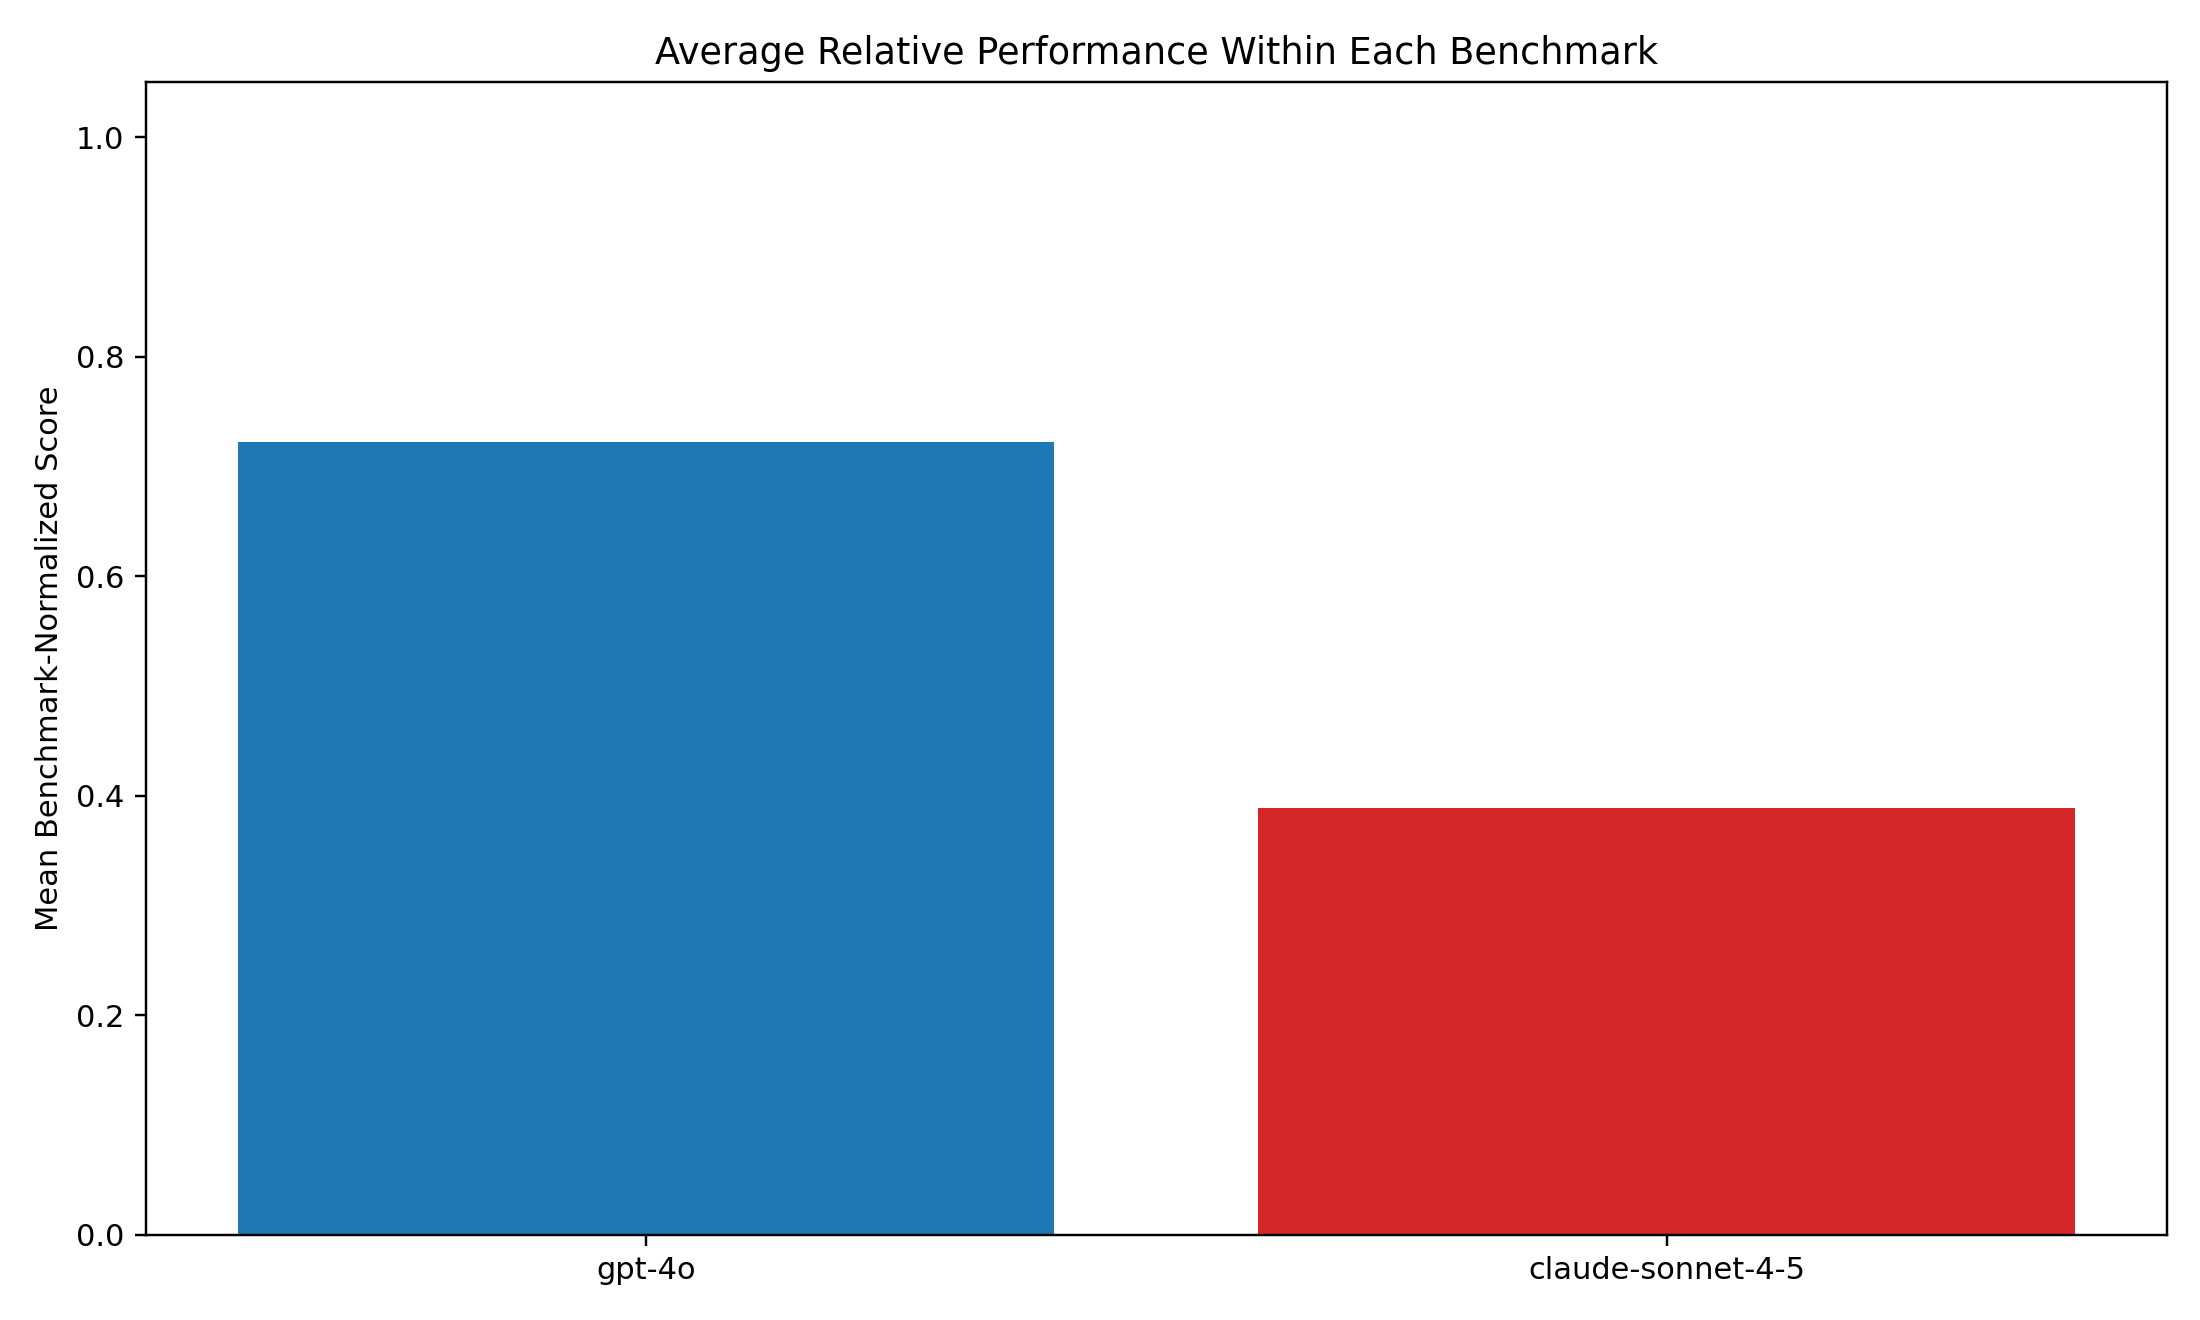
\includegraphics[width=0.78\textwidth]{../../comparison/output/gpt4o_vs_claude/model_normalized_scores.png}
\caption{Mean score normalized within each matched benchmark. GPT-4o wins
more of the benchmark-level comparisons, although the magnitude of the
advantage varies substantially.}
\label{fig:gpt4o-claude-normalized}
\end{figure}

\subsection{Results by Task Family}

\begin{table}[H]
\centering
\small
\caption{Mean primary score by benchmark family. Bold values indicate the
higher raw family mean.}
\label{tab:gpt4o-claude-families}
\begin{tabularx}{\textwidth}{@{}Xrrr@{}}
\toprule
\textbf{Family} & \textbf{Benchmarks} & \textbf{GPT-4o} &
\textbf{Claude Sonnet 4.5} \\
\midrule
Captioning & 10 & \textbf{0.165} & 0.116 \\
Visual question answering & 6 & \textbf{0.800} & 0.508 \\
Labeling & 7 & 0.400 & \textbf{0.436} \\
Detection & 6 & 0.100 & \textbf{0.135} \\
Image modification VQA & 4 & \textbf{0.775} & 0.713 \\
Prompt reconstruction & 3 & 0.833 & \textbf{0.967} \\
\bottomrule
\end{tabularx}
\end{table}

The clearest GPT-4o advantage appears in visual question answering. It leads
on all six QA benchmarks and raises the family mean from 0.508 to 0.800.
The largest individual gaps are ImageNet-1K (0.65 versus 0.15),
FlyingThings3D (0.45 versus 0.00), DocVQA (0.90 versus 0.45),
Fashion-MNIST (0.90 versus 0.55), and GQA (0.80 versus 0.50).
GPT-4o also has the higher captioning and image-modification family means.

The QA result is difficult to dismiss as a single-dataset accident because
the advantage appears on every benchmark in the family. It also spans rather
different visual demands: document reading, object and scene recognition,
spatial reasoning, and conventional question answering. This suggests that
GPT-4o is not merely matching one dataset's answer style. It appears better
at converting visual evidence into the short, evaluator-compatible answer
expected by these tasks. That last qualification is important. A benchmark
rewards both understanding and disciplined output formatting, and the present
experiment cannot completely separate the two.

Captioning presents a similar but less dramatic pattern. GPT-4o's family mean
is higher, yet both absolute means are low because exact n-gram overlap is a
harsh way to judge an open-ended description. A perfectly sensible caption
can use different words from the reference and receive little BLEU credit.
The result therefore supports GPT-4o as the better benchmark captioner in
this experiment, but not necessarily as the model whose prose a human reader
would always prefer. This is one of those places where the metric is useful,
but it is not the whole story.

Claude Sonnet 4.5 is stronger on prompt reconstruction, scoring 1.00 on
ShareGPT-4o-Image compared with 0.70 for GPT-4o, and slightly exceeding
GPT-4o on DiffusionDB and BLIP3o-60k. Its labeling advantage is dominated by
LSUN, where Claude scores 0.95 and GPT-4o scores 0.00. Claude also obtains
higher mean detection F1, including 0.20 scores on Flickr30k Entities and
iNaturalist Detection where GPT-4o scores zero. However, GPT-4o wins more
detection benchmarks overall; this illustrates why win counts and score
magnitudes should be reported together.

Claude's prompt-reconstruction performance is its clearest practical selling
point in this comparison. The task asks the model to infer language that could
have produced or described an image, rather than to select a compact class
label. Claude's strong result may therefore reflect an advantage when visual
analysis has to be turned back into detailed natural language. The family
contains only three benchmarks, so this should be treated as a strong signal
rather than a final verdict, but the consistency across all three is notable.

The LSUN result deserves special attention because a 0.95 versus 0.00 reversal
is large enough to move an entire family average. There are at least two
plausible readings. Claude may genuinely recognize the LSUN scene categories
far more reliably, or GPT-4o may be producing labels that are semantically
reasonable but incompatible with the exact parser or class vocabulary. The
same concern applies to zero-valued detection results, where malformed box
syntax can erase evidence of partial visual understanding. Without a manual
error audit, the honest conclusion is that Claude integrates better with the
current evaluation protocol on those datasets. Claiming that the score proves
a complete absence of visual understanding would go too far.

The image-modification VQA family is more competitive. GPT-4o leads by 0.062
on the family mean, a useful but much smaller advantage than in QA. For a
workflow centred on identifying edits or comparing related images, either
model could therefore be defensible. The wider result favours GPT-4o, while
Claude's prompt-reconstruction strength may matter more when the required
output is descriptive rather than a fixed answer.

\begin{figure}[H]
\centering
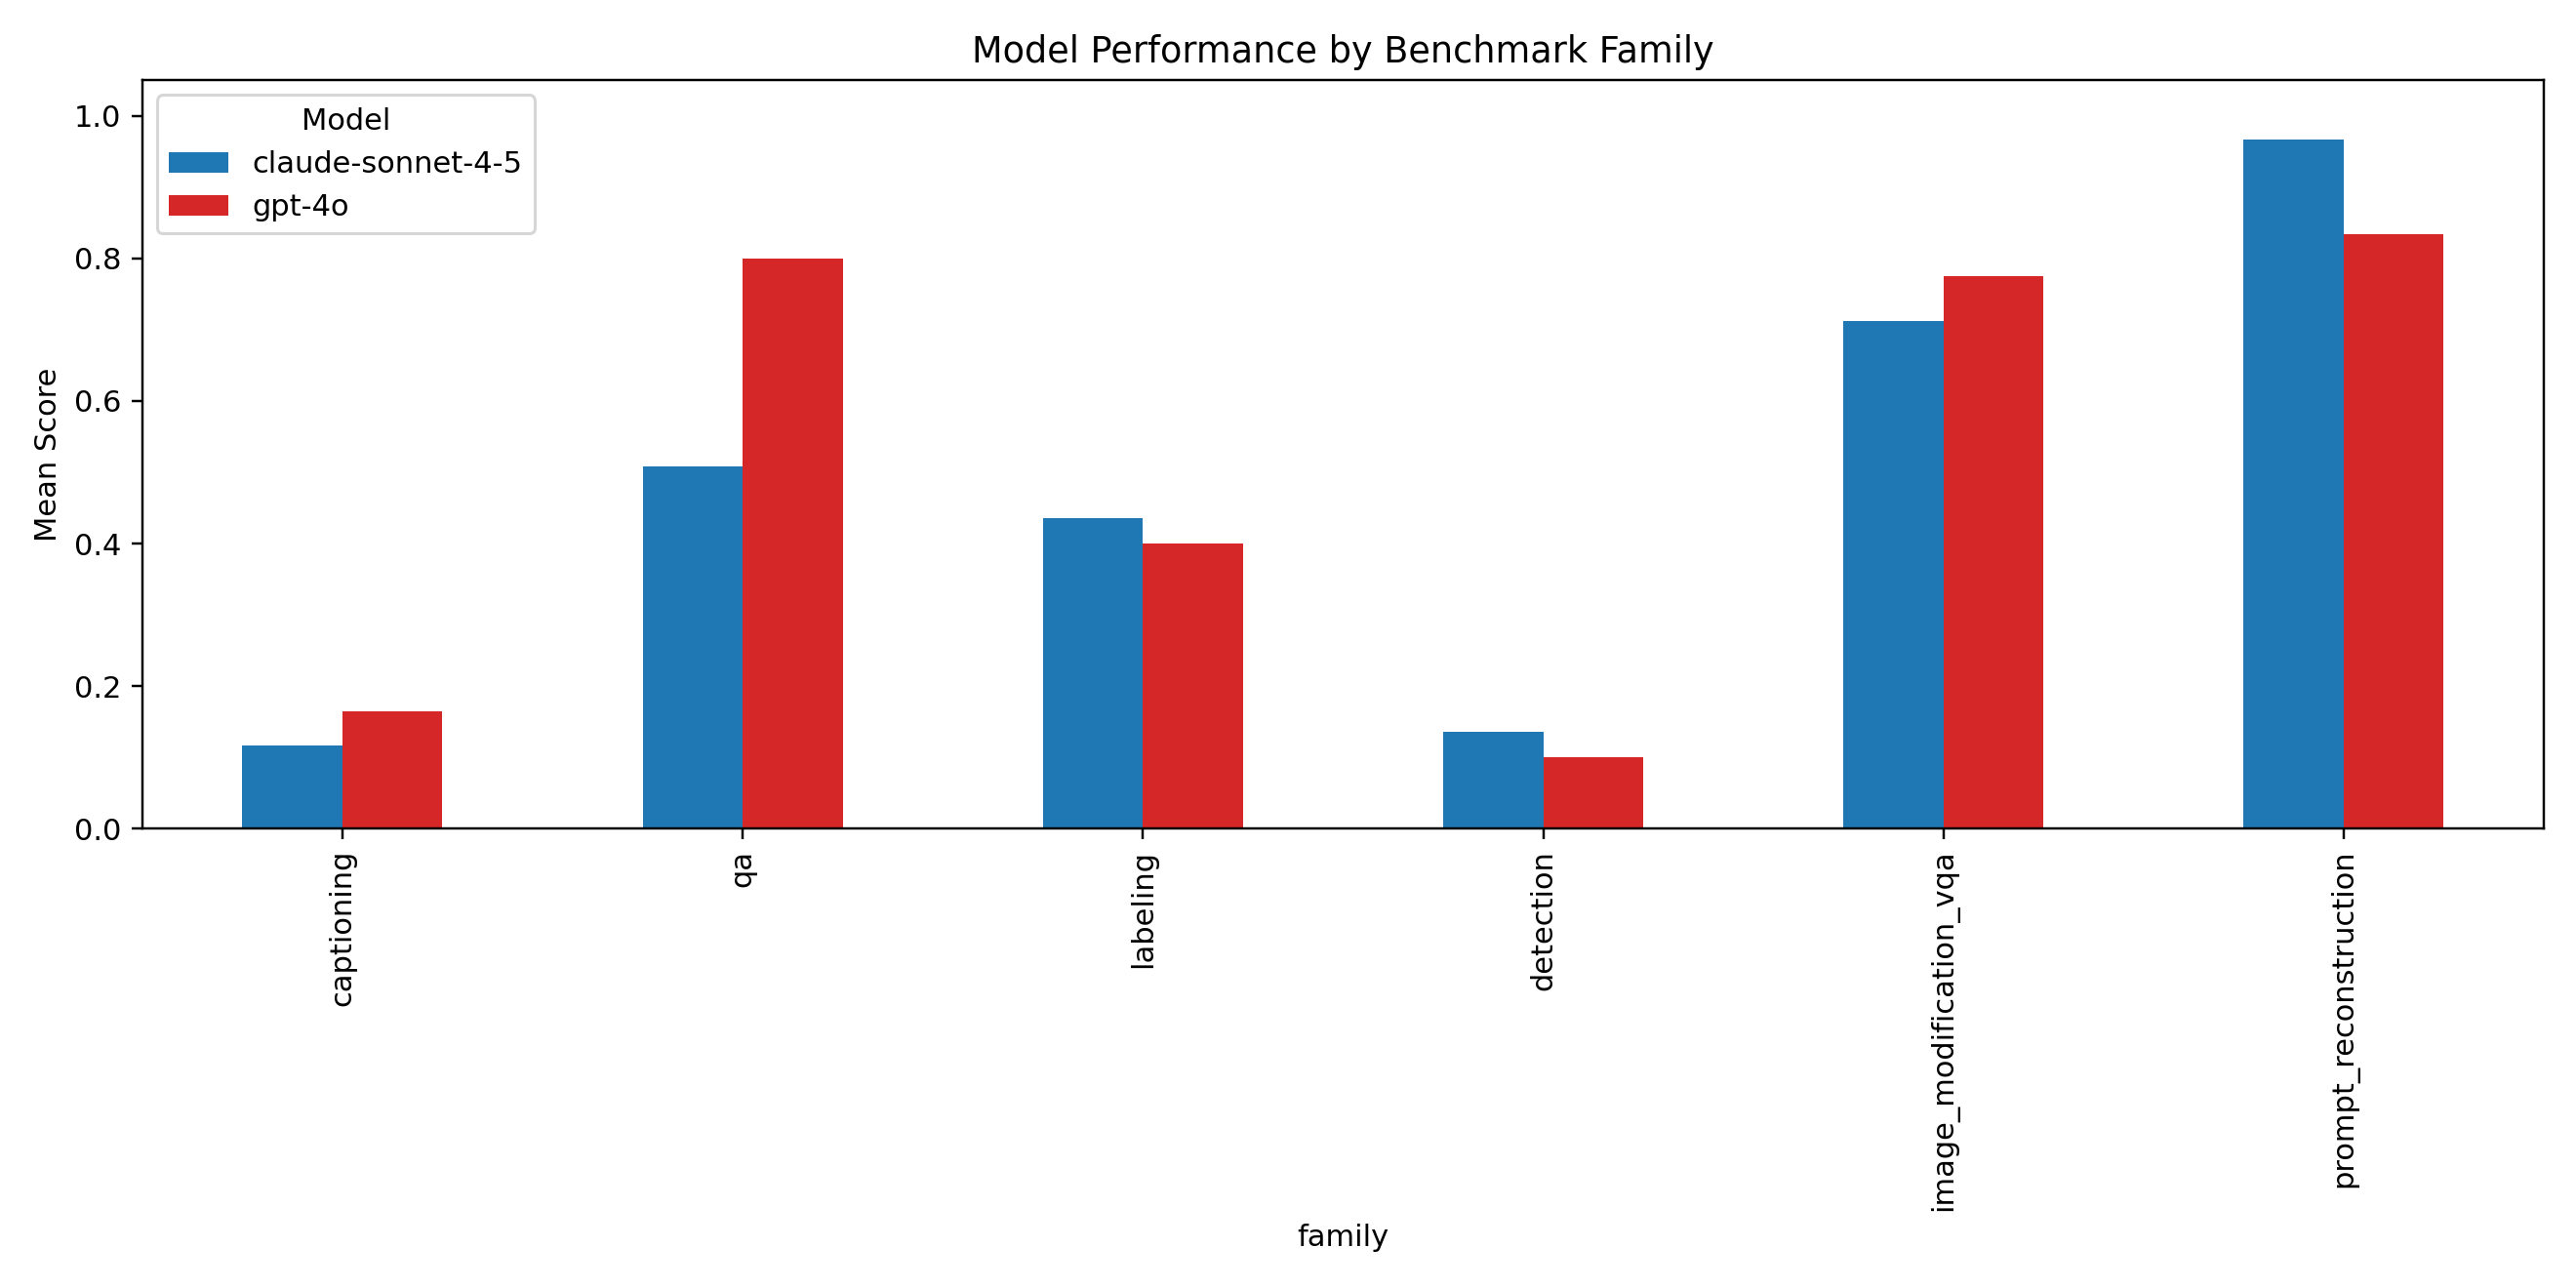
\includegraphics[width=0.88\textwidth]{../../comparison/output/gpt4o_vs_claude/family_grouped_bars.png}
\caption{Raw mean primary score by task family. Metrics differ between
families, so comparisons should be made between models within each family,
not between the heights of unrelated families.}
\label{fig:gpt4o-claude-families}
\end{figure}

\begin{figure}[H]
\centering
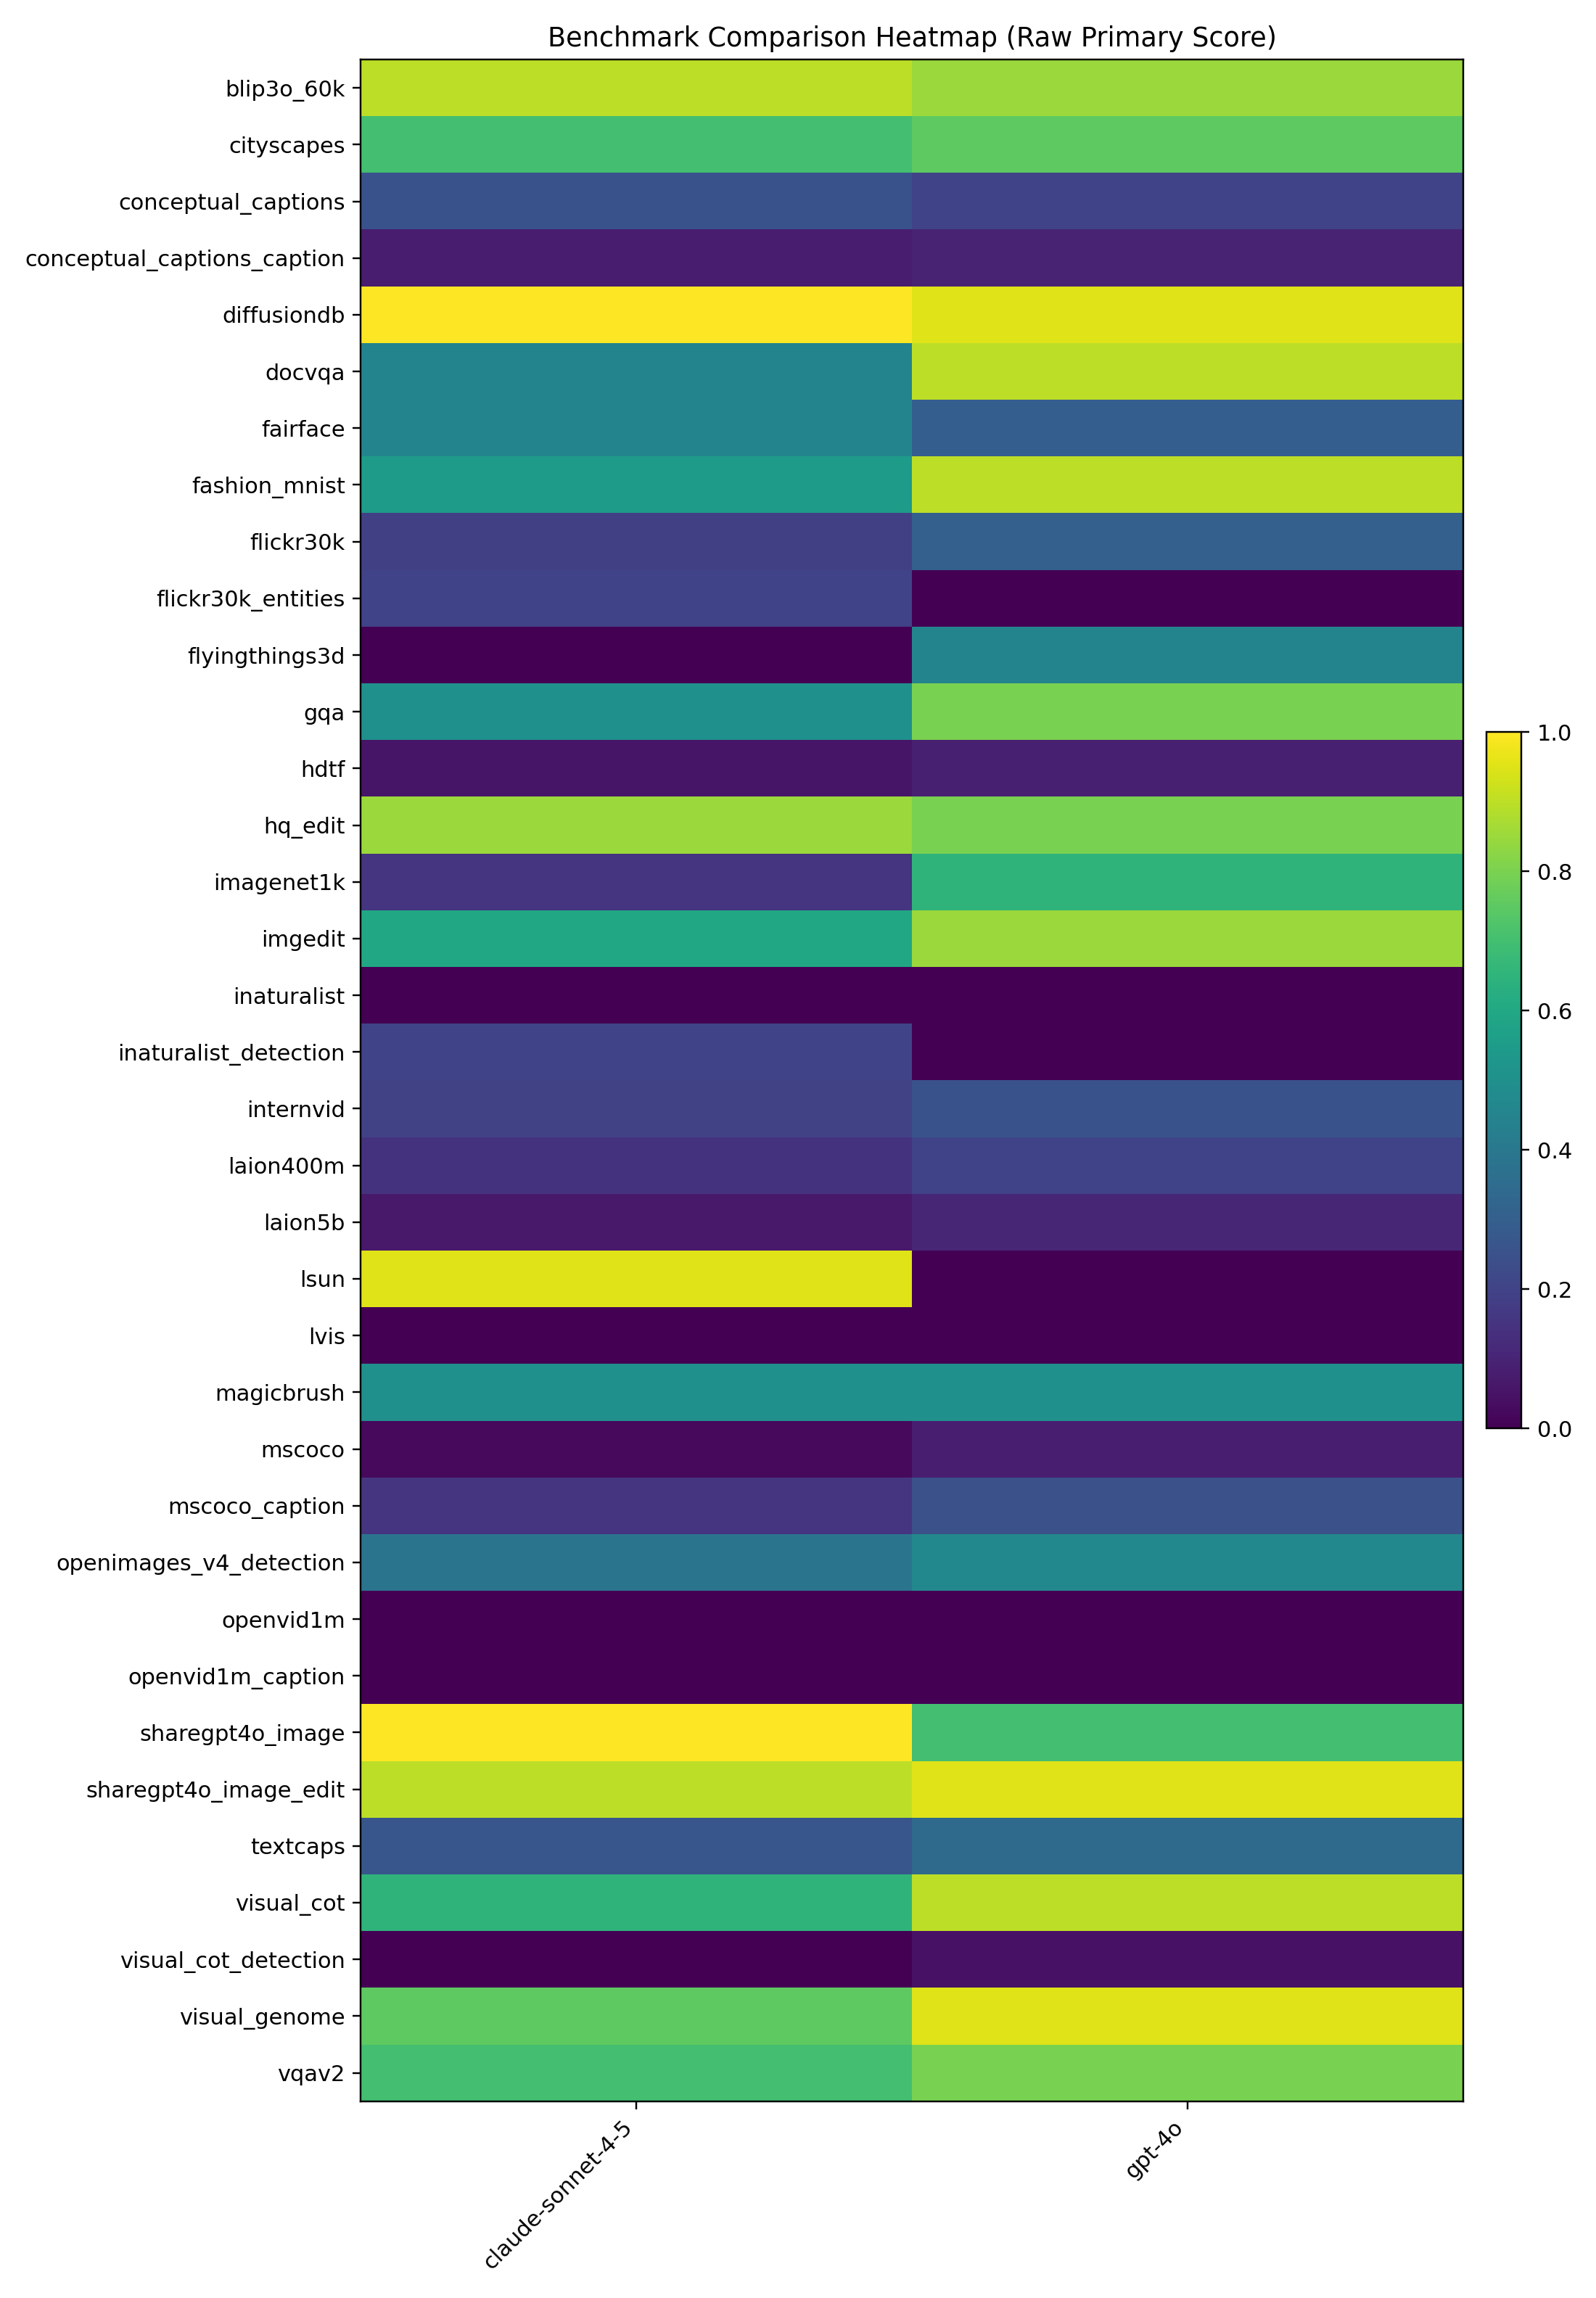
\includegraphics[width=0.82\textwidth]{../../comparison/output/gpt4o_vs_claude/score_heatmap_raw.png}
\caption{Primary score for every matched benchmark. The heatmap exposes
isolated reversals such as Claude's LSUN result that are hidden by aggregate
means.}
\label{fig:gpt4o-claude-heatmap}
\end{figure}

\subsection{Uncertainty and Robustness}

A paired bootstrap was performed by resampling the 36 matched benchmarks
50,000 times. For the difference Claude minus GPT-4o, the observed mean is
\(-0.045\), the 90\% interval is \([-0.108, 0.025]\), and the 95\% interval is
\([-0.120, 0.039]\). Only 13.5\% of bootstrap samples place Claude's mean
above GPT-4o's, equivalent to an estimated 86.5\% probability that GPT-4o
has the higher mean on a resampled benchmark set.

The intervals still cross zero. The evidence therefore supports GPT-4o as
the better model on this particular matched suite, but it does not establish
a conventionally significant universal advantage. The result is sensitive
to benchmark composition and to high-magnitude reversals such as LSUN.
Increasing the sample count per benchmark and completing the remaining
matched datasets would reduce this uncertainty.

This distinction between ``best observed'' and ``proven universally better''
is not just statistical politeness. The benchmark is the unit resampled by
the bootstrap, so the interval asks what might happen if a somewhat different
collection of tasks had been selected. In 13.5\% of those resamples Claude
comes out ahead. That is not the most likely outcome, but it is far from
impossible. The practical reading is that GPT-4o is the stronger default for
the tested workload, whereas a specialised workload should still be tested
directly, especially if it resembles prompt reconstruction, LSUN labeling,
or the detection datasets where Claude recorded larger gains.

There is also uncertainty within each benchmark. Only 20 examples were used,
so one additional correct response changes an accuracy score by 0.05. Several
reported model gaps are exactly that size or smaller. Those close results
should be regarded as near-ties, even when the ranking code must place one
model first. Larger gaps, such as the QA differences listed above, are much
less likely to be explained by one fortunate example.

\subsection{Execution Time}

\begin{table}[H]
\centering
\small
\caption{Measured runtime telemetry over the matched benchmark set.}
\label{tab:gpt4o-claude-runtime}
\begin{tabularx}{\textwidth}{@{}Xrrr@{}}
\toprule
\textbf{Model} & \textbf{Mean wall time/sample} &
\textbf{Mean generation time/sample} & \textbf{Peak CPU RAM} \\
\midrule
\texttt{gpt-4o} & 7.20 s & 4.27 s & 1.99 GiB \\
\texttt{claude-sonnet-4-5} & 8.07 s & 3.94 s & 1.86 GiB \\
\bottomrule
\end{tabularx}
\end{table}

GPT-4o has approximately 10.8\% lower end-to-end wall-clock latency, despite
Claude recording slightly lower model-generation time. The difference
indicates that network, request preparation, provider queueing, or response
handling contributes materially to total latency. These values describe the
observed API routes during this run and should not be treated as permanent
provider speed guarantees.

The latency breakdown is a useful reminder that the model's generation time
is not the same as the time experienced by an application. Claude generated
its answer about 0.33 seconds faster on average, yet the complete request took
about 0.87 seconds longer. In an interactive tool, GPT-4o would consequently
feel faster in these runs even though its measured generation stage was
slower. For a large offline batch, the same difference accumulates: over the
720 matched evaluations, the mean wall times correspond to roughly 86
minutes for GPT-4o and 97 minutes for Claude if requests are processed
sequentially.

Neither model has a meaningful local-memory advantage. The 0.13 GiB
difference in peak CPU RAM is small and, for hosted APIs, local memory is
unlikely to be the deployment bottleneck anyway. API price limits, request
rate limits, and wall-clock throughput are more consequential. The timing
comparison should also be viewed as a snapshot: provider load and network
conditions can change from one hour to the next.

\subsection{Validity Limitations}

The comparison uses 20 examples per benchmark, which is sufficient for a
broad diagnostic comparison but not for precise dataset-level estimates.
Captioning, detection, classification, and multiple-choice metrics measure
different properties; averaging them gives every benchmark equal weight but
does not create a single absolute measure of intelligence. Some datasets
also expose formatting sensitivity: a semantically useful response can score
poorly if it does not follow the expected label or bounding-box format.

Finally, the analysis is a snapshot of mutable hosted APIs. Model aliases,
provider infrastructure, safety behaviour, and tokenization may change.
The reproducible artifacts for this comparison are stored in
\texttt{comparison/output/gpt4o\_vs\_claude/}, including benchmark-level
scores, family summaries, pairwise wins, telemetry, plots, and the paired
bootstrap difference. The five-model artifacts are stored in
\texttt{comparison/output/five\_api\_models/}.

One further limitation is that every benchmark receives equal weight in the
aggregate, regardless of its difficulty, sample diversity, or importance to
a real application. This is transparent and avoids choosing weights after
seeing the results, but it is not automatically the right weighting for every
user. A document-processing product might reasonably give DocVQA much more
importance than Fashion-MNIST, while an image-search system might do the
opposite. The aggregate ranking is therefore a useful general-purpose answer,
not a substitute for choosing benchmarks that match the intended deployment.

\section{Five-Model API Comparison}

\subsection{Scope and Overall Ranking}

A second matched comparison uses the 21 benchmarks completed by GPT-4o,
GPT-4.1, GPT-5, Gemini 3.5 Flash, and Claude Sonnet 4.5. The common set
contains 6 QA, 6 detection, and 9 captioning benchmarks, giving 420 evaluated
examples per model. This intersection is smaller than the 36-benchmark
two-model study because a benchmark is admitted only when all five models
have a completed result. The stricter matching makes the comparison fair,
but it also removes labeling, image-modification VQA, and prompt
reconstruction from this particular analysis.

\begin{table}[H]
\centering
\small
\caption{Results over the 21 benchmarks completed by all five API models.}
\label{tab:five-api-models}
\begin{tabularx}{\textwidth}{@{}Xrrrr@{}}
\toprule
\textbf{Model} & \textbf{Mean score} & \textbf{Normalized} &
\textbf{Mean rank} & \textbf{First places} \\
\midrule
\texttt{gpt-4o} & \textbf{0.336} & \textbf{0.803} & \textbf{1.71} & \textbf{12} \\
\texttt{gpt-4.1} & 0.275 & 0.469 & 2.43 & 8 \\
\texttt{gpt-5} & 0.243 & 0.323 & 2.81 & 5 \\
\texttt{claude-sonnet-4-5} & 0.239 & 0.650 & 2.52 & 4 \\
\texttt{gemini-3.5-flash} & 0.025 & 0.157 & 3.33 & 2 \\
\bottomrule
\end{tabularx}
\end{table}

GPT-4o is the clearest all-round performer. It has the highest raw mean, the
highest normalized mean, the best average rank, and the most first-place
finishes. In other words, its lead does not depend on selecting one convenient
summary statistic. It wins or ties for first on 12 of the 21 benchmarks and
its normalized score of 0.803 is well above Claude's second-place 0.650.

The middle of the table is more interesting than a simple reading of the raw
mean suggests. GPT-4.1 has the second-highest raw score and a slightly better
mean rank than Claude, but Claude has a much higher normalized score. GPT-5
also has a marginally higher raw mean than Claude while performing much worse
after within-benchmark normalization. This disagreement occurs because raw
metrics have different scales and because a model can collect a high raw
average from a few high-scoring benchmark types. The normalized result asks
how each model performs relative to the other models on the same benchmark.
On that basis, Claude is the more competitive second-place model, even though
GPT-4.1 reaches first place more often.

This is a useful warning against sorting a heterogeneous benchmark table by
one column and calling the job done. GPT-4.1 appears to have sharper peaks:
it records eight first places and leads the QA family. Claude records only
four first places, but its stronger normalized mean indicates fewer or less
severe relative failures across the common set. Choosing between them depends
on whether a project values peak performance on a target task or steadier
performance across task types.

\subsection{Task Families and Pairwise Behaviour}

GPT-4o leads captioning with a raw family mean of 0.183. GPT-4.1 leads all
models on QA with 0.867, while Claude leads detection with 0.135. The family
winners therefore come from three different models. GPT-4o's overall victory
is not the result of sweeping every category; it comes from combining strong
captioning with competitive results elsewhere. GPT-4.1's QA lead is
especially relevant because the two-model study already identified QA as a
major strength of GPT-4o. On the reduced common set, GPT-4.1 improves even on
that strong baseline.

Claude's detection lead repeats the pattern seen in the broader comparison
with GPT-4o. That repetition makes the finding more credible: detection is
not merely one isolated win hidden inside the larger table. Still, an F1 mean
of 0.135 is low in absolute terms. Claude is best among these APIs under the
current detection prompt and parser, but none of the models should be
described as solving detection reliably. For applications where bounding
boxes are central, a specialised detector remains the more sensible
baseline.

The pairwise results reinforce GPT-4o's position. It beats Gemini on 88.1\%
of matched comparisons, Claude on 83.3\%, and GPT-5 on 71.4\%. Its mean score
advantage is 0.311 over Gemini, 0.096 over Claude, and 0.093 over GPT-5.
These are not all equivalent victories: the Gemini gap is both frequent and
large, whereas the GPT-5 comparison is closer and more dependent on task
composition.

Claude beats GPT-5 on 66.7\% of benchmarks but has a mean raw difference of
\(-0.004\). This apparently contradictory result is actually informative.
Claude wins more often, while GPT-5's less frequent wins are large enough to
erase the average raw advantage. For a broad workload, Claude's consistency
may be preferable. For a narrow workload that happens to match one of
GPT-5's stronger tasks, the aggregate pairwise win rate could be misleading.
The benchmark-level heatmaps and scores should therefore be consulted before
making a deployment decision.

\subsection{Uncertainty}

Bootstrap intervals for the raw mean are broad: GPT-4o scores 0.336 with a
90\% interval of \([0.221, 0.456]\), GPT-4.1 scores 0.275 with
\([0.142, 0.419]\), GPT-5 scores 0.243 with \([0.110, 0.390]\), and Claude
scores 0.239 with \([0.158, 0.326]\). These four intervals overlap heavily.
The observed ordering among the leading models should therefore be understood
as the ranking for this 21-benchmark set, not as a precise universal league
table.

Gemini is the exception. Its raw mean is 0.025 with a 90\% interval of
\([0.009, 0.044]\), which does not overlap the intervals of the other four
models. Its weak result is consequently more stable than the exact ordering
within the leading group. Even here, some caution is needed: a consistently
low score can indicate weak visual-task performance, but it can also reveal a
systematic mismatch between the model's response format and the evaluator.
A manual review of Gemini's failed samples would be required to separate
those explanations.

The smaller benchmark intersection also changes the question being answered.
This study says how the five models compare on captioning, QA, and detection.
It says nothing directly about their relative labeling or prompt-
reconstruction ability. That matters because prompt reconstruction is where
Claude was strongest in the broader two-model study. The five-model ranking
should not be extrapolated to families that it never tested.

\subsection{Runtime and Practical Trade-offs}

\begin{table}[H]
\centering
\small
\caption{Measured runtime telemetry over the 21 benchmarks shared by all five
models.}
\label{tab:five-api-runtime}
\begin{tabularx}{\textwidth}{@{}Xrrr@{}}
\toprule
\textbf{Model} & \textbf{Wall time/sample} &
\textbf{Generation time/sample} & \textbf{Peak CPU RAM} \\
\midrule
\texttt{gpt-4o} & 8.67 s & 3.81 s & 1.99 GiB \\
\texttt{claude-sonnet-4-5} & 10.19 s & 3.38 s & 1.86 GiB \\
\texttt{gpt-4.1} & 10.74 s & 2.94 s & 1.58 GiB \\
\texttt{gpt-5} & 11.17 s & 3.23 s & 1.44 GiB \\
\texttt{gemini-3.5-flash} & 19.13 s & 10.56 s & 1.56 GiB \\
\bottomrule
\end{tabularx}
\end{table}

GPT-4o is fastest end to end at 8.67 seconds per sample, despite GPT-4.1
having the shortest measured generation stage. This repeats the lesson from
the two-model study: provider overhead is a substantial part of API latency.
GPT-4.1 generates in 2.94 seconds but takes 10.74 seconds overall, leaving
roughly 7.8 seconds in upload, queueing, network transfer, preprocessing, or
response handling. A fast decoder does not automatically produce a fast user
experience.

Gemini is the clear runtime outlier at 19.13 seconds per sample, more than
twice GPT-4o's wall time, and it also has by far the longest generation time.
Combined with its low benchmark score, this run gives no accuracy--latency
trade-off in Gemini's favour. The result may still reflect a provider route,
region, or account configuration rather than a permanent property of the
model, so it should be remeasured before a production decision.

Local peak RAM ranges only from 1.44 to 1.99 GiB and is unlikely to determine
the API-model choice. The meaningful practical trade-off is between task
quality, latency, and price. GPT-4o offers the best quality and wall time in
this experiment. GPT-4.1 is attractive for QA, Claude for detection and
cross-task consistency, and GPT-5 shows occasional strong wins without
matching GPT-4o overall. Model routing by task could therefore outperform a
single-model policy, although it would add implementation complexity and
require enough traffic to justify maintaining several providers.

\begin{figure}[H]
\centering
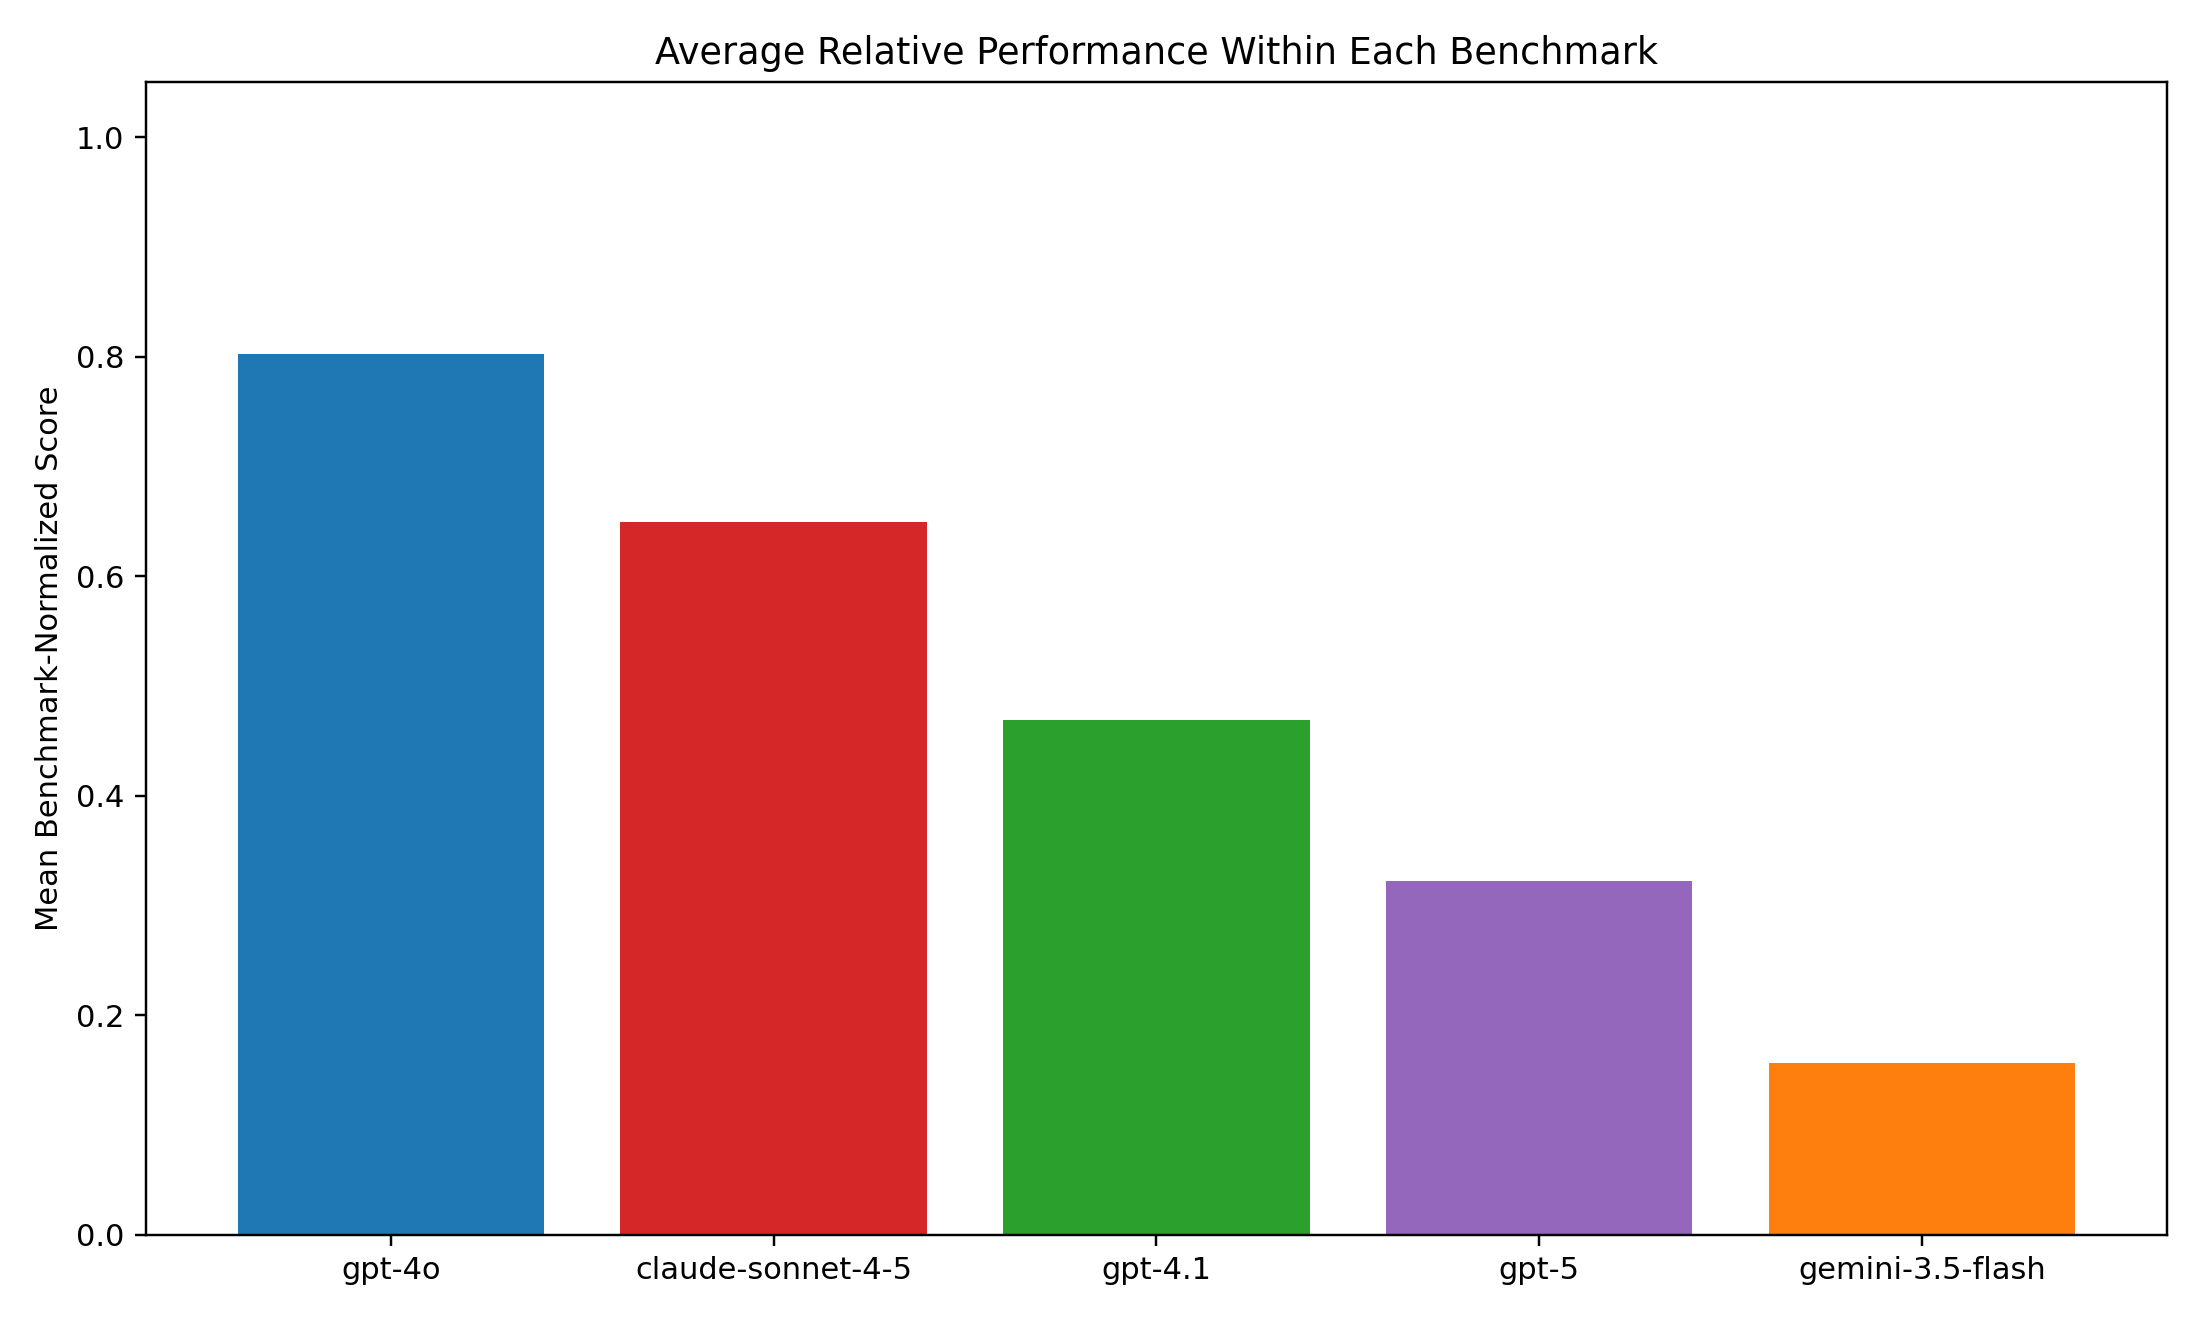
\includegraphics[width=0.82\textwidth]{../../comparison/output/five_api_models/model_normalized_scores.png}
\caption{Mean benchmark-normalized score across the 21 matched benchmarks.}
\label{fig:five-api-models}
\end{figure}

\subsection{Overall Interpretation}

Taken together, the five-model experiment supports GPT-4o as the best default
for the benchmark mix studied here. That conclusion is straightforward.
The more useful secondary conclusion is that there is no universal runner-up.
Claude looks strongest after benchmark normalization, GPT-4.1 has the best
QA mean and more first-place finishes, and GPT-5 is close to Claude in raw
mean while behaving less consistently. The right second choice therefore
depends on the workload rather than on a single overall number.

The study also shows why the broader GPT-4o--Claude comparison remains
necessary. Restricting the data to what every model completed makes a clean
five-way comparison possible, but it throws away 15 matched benchmarks and
three entire task families available for those two models. The 36-benchmark
study gives the more complete answer when choosing specifically between
GPT-4o and Claude; the 21-benchmark study gives the fairer answer when all
five systems must be considered together. Neither replaces the other.

\section{Conclusions and Future Work}

This project produced a common and reproducible framework for evaluating
vision-language models across a broad collection of datasets and task types.
The same model interface, prompts, sample counts, metrics, and telemetry were
used throughout, allowing hosted models from different providers to be
compared under reasonably consistent conditions.

Across the 36 benchmarks shared by GPT-4o and Claude Sonnet 4.5, GPT-4o was
the stronger general-purpose model. It won more benchmarks, achieved the
higher normalized score, and performed particularly well in visual question
answering and captioning. Claude remained competitive and was notably stronger
in prompt reconstruction and some detection and labeling tasks. The result is
therefore not that one model is always better, but that GPT-4o is the safer
default while Claude may be preferable for particular workloads.

The five-model comparison reached a similar overall conclusion. GPT-4o led
the 21-benchmark common set and also had the lowest observed end-to-end
latency. GPT-4.1 produced the best QA mean, while Claude obtained the best
detection mean. GPT-5 showed occasional strong results but was less consistent,
and Gemini 3.5 Flash performed poorly under the current prompts and evaluation
format. In practice, routing tasks to specialised models could outperform
using one model for everything, although it would make the system more complex
and expensive to maintain.

These findings must be read with the limitations of the experiment in mind.
Only 20 examples were evaluated per benchmark, the metrics are heterogeneous,
and hosted APIs can change without notice. Some low scores may also reflect
strict output parsing rather than a complete failure of visual understanding.
The results are consequently a useful experimental snapshot, not a permanent
leaderboard.

Future work should increase the number of samples, manually inspect formatting
failures, test for benchmark contamination, and repeat the measurements over
time. It would also be useful to complete the missing model--dataset
combinations and compare API systems with locally hosted and fine-tuned
vision-language models. Even with its limitations, the study demonstrates a
clear point: model quality cannot be represented fairly by one benchmark or
one average. The task, metric, latency, cost, and deployment context all matter.

\clearpage
\section{References}
\begin{thebibliography}{99}
\bibitem{vaswani2017attention} A. Vaswani et al., ``Attention Is All You Need,'' NeurIPS, 2017. \url{https://arxiv.org/abs/1706.03762}.
\bibitem{hendrycks2020mmlu} D. Hendrycks et al., ``Measuring Massive Multitask Language Understanding,'' ICLR, 2021. \url{https://arxiv.org/abs/2009.03300}.
\bibitem{kiela2021dynabench} D. Kiela et al., ``Dynabench: Rethinking Benchmarking in NLP,'' NAACL, 2021. \url{https://arxiv.org/abs/2104.14337}.
\bibitem{srivastava2022bigbench} A. Srivastava et al., ``Beyond the Imitation Game: Quantifying and Extrapolating the Capabilities of Language Models,'' Transactions on Machine Learning Research, 2023. \url{https://arxiv.org/abs/2206.04615}.
\bibitem{liang2022helm} P. Liang et al., ``Holistic Evaluation of Language Models,'' Transactions on Machine Learning Research, 2023. \url{https://arxiv.org/abs/2211.09110}.
\bibitem{yue2023mmmu} X. Yue et al., ``MMMU: A Massive Multi-discipline Multimodal Understanding and Reasoning Benchmark for Expert AGI,'' CVPR, 2024. \url{https://arxiv.org/abs/2311.16502}.
\bibitem{reddi2019mlperf} V. J. Reddi et al., ``MLPerf Inference Benchmark,'' ISCA, 2020. \url{https://arxiv.org/abs/1911.02549}.
\bibitem{li2023contamination} Y. Li, F. Guerin, and C. Lin, ``An Open Source Data Contamination Report for Large Language Models,'' 2023. \url{https://arxiv.org/abs/2310.17589}.
\bibitem{deng2009imagenet} J. Deng et al., ``ImageNet: A Large-Scale Hierarchical Image Database,'' CVPR, 2009. \url{https://doi.org/10.1109/CVPR.2009.5206848}.
\bibitem{soomro2012ucf101} K. Soomro, A. R. Zamir, and M. Shah, ``UCF101: A Dataset of 101 Human Actions Classes From Videos in the Wild,'' 2012. \url{https://arxiv.org/abs/1212.0402}.
\bibitem{lin2014coco} T.-Y. Lin et al., ``Microsoft COCO: Common Objects in Context,'' ECCV, 2014. \url{https://arxiv.org/abs/1405.0312}.
\bibitem{plummer2015flickr30k} B. A. Plummer et al., ``Flickr30k Entities: Collecting Region-to-Phrase Correspondences for Richer Image-to-Sentence Models,'' ICCV, 2015. \url{https://arxiv.org/abs/1505.04870}.
\bibitem{mayer2016large} N. Mayer et al., ``A Large Dataset to Train Convolutional Networks for Disparity, Optical Flow, and Scene Flow Estimation,'' CVPR, 2016. \url{https://arxiv.org/abs/1512.02134}.
\bibitem{yu2015lsun} F. Yu et al., ``LSUN: Construction of a Large-scale Image Dataset using Deep Learning with Humans in the Loop,'' 2015. \url{https://arxiv.org/abs/1506.03365}.
\bibitem{cordts2016cityscapes} M. Cordts et al., ``The Cityscapes Dataset for Semantic Urban Scene Understanding,'' CVPR, 2016. \url{https://arxiv.org/abs/1604.01685}.
\bibitem{krishna2017visualgenome} R. Krishna et al., ``Visual Genome: Connecting Language and Vision Using Crowdsourced Dense Image Annotations,'' IJCV, 2017. \url{https://arxiv.org/abs/1602.07332}.
\bibitem{goyal2017vqa} Y. Goyal et al., ``Making the V in VQA Matter,'' CVPR, 2017. \url{https://arxiv.org/abs/1612.00837}.
\bibitem{xiao2017fashionmnist} H. Xiao, K. Rasul, and R. Vollgraf, ``Fashion-MNIST: a Novel Image Dataset for Benchmarking Machine Learning Algorithms,'' 2017. \url{https://arxiv.org/abs/1708.07747}.
\bibitem{kay2017kinetics} W. Kay et al., ``The Kinetics Human Action Video Dataset,'' 2017. \url{https://arxiv.org/abs/1705.06950}.
\bibitem{vanhorn2018inaturalist} G. Van Horn et al., ``The iNaturalist Species Classification and Detection Dataset,'' CVPR, 2018. \url{https://arxiv.org/abs/1707.06642}.
\bibitem{zhou2017places} B. Zhou et al., ``Places: A 10 Million Image Database for Scene Recognition,'' TPAMI, 2017. \url{https://arxiv.org/abs/1610.02055}.
\bibitem{sharma2018conceptual} P. Sharma et al., ``Conceptual Captions: A Cleaned, Hypernymed, Image Alt-text Dataset for Automatic Image Captioning,'' ACL, 2018. \url{https://aclanthology.org/P18-1238/}.
\bibitem{kuznetsova2020openimages} A. Kuznetsova et al., ``The Open Images Dataset V4,'' IJCV, 2020. \url{https://arxiv.org/abs/1811.00982}.
\bibitem{hudson2019gqa} D. A. Hudson and C. D. Manning, ``GQA: A New Dataset for Real-World Visual Reasoning and Compositional Question Answering,'' CVPR, 2019. \url{https://arxiv.org/abs/1902.09506}.
\bibitem{bergmann2019mvtec} P. Bergmann et al., ``MVTec AD---A Comprehensive Real-World Dataset for Unsupervised Anomaly Detection,'' CVPR, 2019. \url{https://arxiv.org/abs/1904.09665}.
\bibitem{gupta2019lvis} A. Gupta, P. Dollar, and R. Girshick, ``LVIS: A Dataset for Large Vocabulary Instance Segmentation,'' CVPR, 2019. \url{https://arxiv.org/abs/1908.03195}.
\bibitem{mathew2020docvqa} M. Mathew, D. Karatzas, and C. V. Jawahar, ``DocVQA: A Dataset for VQA on Document Images,'' WACV, 2021. \url{https://arxiv.org/abs/2007.00398}.
\bibitem{dolhansky2020dfdc} B. Dolhansky et al., ``The DeepFake Detection Challenge (DFDC) Dataset,'' 2020. \url{https://arxiv.org/abs/2006.07397}.
\bibitem{sidorov2020textcaps} O. Sidorov et al., ``TextCaps: a Dataset for Image Captioning with Reading Comprehension,'' ECCV, 2020. \url{https://arxiv.org/abs/2003.12462}.
\bibitem{schuhmann2021laion400m} C. Schuhmann et al., ``LAION-400M: Open Dataset of CLIP-Filtered 400 Million Image-Text Pairs,'' 2021. \url{https://arxiv.org/abs/2111.02114}.
\bibitem{karkkainen2021fairface} K. Karkkainen and J. Joo, ``FairFace: Face Attribute Dataset for Balanced Race, Gender, and Age,'' WACV, 2021. \url{https://arxiv.org/abs/1908.04913}.
\bibitem{zhang2021hdtf} Z. Zhang et al., ``Flow-guided One-shot Talking Face Generation with a High-Definition Talking Face Dataset,'' CVPR, 2021. \url{https://github.com/MRzzm/HDTF}.
\bibitem{schuhmann2022laion5b} C. Schuhmann et al., ``LAION-5B: An Open Large-Scale Dataset for Training Next Generation Image-Text Models,'' NeurIPS Datasets and Benchmarks, 2022. \url{https://arxiv.org/abs/2210.08402}.
\bibitem{wang2022diffusiondb} Z. J. Wang et al., ``DiffusionDB: A Large-scale Prompt Gallery Dataset for Text-to-Image Generative Models,'' ACL, 2023. \url{https://arxiv.org/abs/2210.14896}.
\bibitem{he2022tad66k} S. He et al., ``Theme-Aware Visual Attribute Reasoning for Image Aesthetics Assessment,'' ACM MM, 2022. \url{https://github.com/woshidandan/TANet}.
\bibitem{zhang2023magicbrush} K. Zhang et al., ``MagicBrush: A Manually Annotated Dataset for Instruction-Guided Image Editing,'' NeurIPS Datasets and Benchmarks, 2023. \url{https://arxiv.org/abs/2306.10012}.
\bibitem{kirstain2023pickapic} Y. Kirstain et al., ``Pick-a-Pic: An Open Dataset of User Preferences for Text-to-Image Generation,'' NeurIPS, 2023. \url{https://arxiv.org/abs/2305.01569}.
\bibitem{wang2023internvid} Y. Wang et al., ``InternVid: A Large-scale Video-Text Dataset for Multimodal Understanding and Generation,'' 2023. \url{https://arxiv.org/abs/2307.06942}.
\bibitem{nan2024openvid} K. Nan et al., ``OpenVid-1M: A Large-Scale High-Quality Dataset for Text-to-video Generation,'' 2024. \url{https://arxiv.org/abs/2407.02371}.
\bibitem{shao2024visualcot} H. Shao et al., ``Visual CoT: Advancing Multi-Modal Language Models with a Comprehensive Dataset and Benchmark for Chain-of-Thought Reasoning,'' 2024. \url{https://arxiv.org/abs/2403.16999}.
\bibitem{hui2024hqedit} M. Hui et al., ``HQ-Edit: A High-Quality Dataset for Instruction-based Image Editing,'' 2024. \url{https://arxiv.org/abs/2404.09990}.
\bibitem{chen2025blip3o} J. Chen et al., ``BLIP3-o: A Family of Fully Open Unified Multimodal Models---Architecture, Training and Dataset,'' 2025. \url{https://arxiv.org/abs/2505.09568}.
\bibitem{ye2025imgedit} Y. Ye et al., ``ImgEdit: A Unified Image Editing Dataset and Benchmark,'' 2025. \url{https://arxiv.org/abs/2505.20275}.
\bibitem{chen2025sharegpt} J. Chen et al., ``ShareGPT-4o-Image: Aligning Multimodal Models with GPT-4o-Level Image Generation,'' 2025. \url{https://arxiv.org/abs/2506.18095}.
\bibitem{kinney2023semanticscholar} R. Kinney et al., ``The Semantic Scholar Open Data Platform,'' 2023. \url{https://arxiv.org/abs/2301.10140}.
\bibitem{yue2024mmmupro} X. Yue et al., ``MMMU-Pro: A More Robust Multi-discipline Multimodal Understanding Benchmark,'' 2024. \url{https://arxiv.org/abs/2409.02813}.
\bibitem{chiang2024arena} W.-L. Chiang et al., ``Chatbot Arena: An Open Platform for Evaluating LLMs by Human Preference,'' ICML, 2024. \url{https://arxiv.org/abs/2403.04132}.
\bibitem{lmarenaVision} LM Arena, ``Vision Arena Leaderboard.'' \url{https://lmarena.ai/leaderboard/vision}. Accessed June 10, 2026.
\bibitem{nvidiaB300} NVIDIA, ``NVIDIA B300 Tensor Core GPU.'' \url{https://www.nvidia.com/en-us/data-center/b300/}. Accessed June 10, 2026.
\end{thebibliography}

\clearpage
\appendix
\end{document}

